\chapter{Fractions et\\décimaux} \label{Num4}
 
 
\begin{prerequis}[Dans les programmes - cycle 3]
{\bf Utiliser et représenter des fractions simples, les nombres décimaux}
   \begin{itemize}
      \item Connaître diverses désignations des fractions : orales, écrites et décompositions additives et multiplicatives (ex : quatre tiers ; $\frac 43 ; \frac13+\frac13+\frac13+\frac13 ; 1+\frac13 ; 4 \times \frac13$).
      \item Connaître et utiliser quelques fractions simples comme opérateur de partage en faisant le lien entre les formulations en langage courant et leur écriture mathématique (ex : faire le lien entre \og la moitié de \fg{} et multiplier par $\frac12$).
      \item Utiliser des fractions pour rendre compte de partages de grandeurs ou de mesures de grandeurs. Repérer et placer des fractions sur une demi-droite graduée adaptée.
      \item Encadrer une fraction par deux nombres entiers consécutifs. Comparer deux fractions de même dénominateur.
      \item Écrire une fraction sous forme de somme d’un entier et d’une fraction inférieure à 1. Connaître des égalités entre des fractions usuelles (ex : $\frac5{10} =\frac12 ; \frac{10}{100} =\frac1{10} ; \frac24 =\frac12$). Utiliser des fractions pour exprimer un quotient.
      \item Connaître les unités de la numération décimale (unités simples, dixièmes, centièmes, millièmes) et les relations qui les lient.
      \item Comprendre et appliquer aux nombres décimaux les règles de la numération décimale de position (valeurs des chiffres en fonction de leur rang).
      \item Connaître et utiliser diverses désignations orales et écrites d’un nombre décimal (fractions décimales, écritures à virgule, décompositions additives et multiplicatives).
      \item Utiliser les nombres décimaux pour rendre compte de mesures de grandeurs.
      \item Connaître le lien entre les unités de numération et les unités de mesure (par exemple : dixième à dm/dg/dL, centième à cm/cg/cL/centimes d’euro).
      \item Repérer et placer un nombre décimal sur une demi-droite graduée adaptée. Comparer, ranger des nombres décimaux.
      \item Encadrer un nombre décimal par deux nombres entiers, par deux nombres décimaux.
      \item Trouver des nombres décimaux à intercaler entre deux nombres donnés.
   \end{itemize}
\end{prerequis}


%%%%%%%%%%%%%%%%%%%%%%%%%
%%%%%%%%%%%%%%%%%%%%%%%%%
\reperes 

%%%%%%%%%%
\section{Introduction}
%%%%%%%%%% 


\subsection{Repères de progressivité}

Les fractions, puis les nombres décimaux, apparaissent comme de nouveaux nombres introduits pour pallier l’insuffisance des nombres entiers, notamment pour mesurer des longueurs, des aires et repérer des points sur une demi-droite graduée. Le lien à établir avec les connaissances acquises à propos des entiers est essentiel. Avoir une bonne compréhension des relations entre les différentes unités de numération des entiers (unités, dizaines, centaines de chaque ordre) permet de les prolonger aux dixièmes, centièmes\dots{} L’écriture à virgule est présentée comme une convention d’écriture d’une fraction décimale ou d’une somme de fractions décimales. Cela permet de mettre à jour la nature des nombres décimaux et de justifier les règles de comparaison et de calcul. 

Au {\bf CM1}, dès la période 1, les élèves utilisent les fractions simples comme $\frac23, \frac12, \frac52$ (il est important de travailler les\\[1mm]fractions inférieures et supérieures à l'unité) dans le cadre de partage de grandeurs. \\
En période 2, ils mobilisent les fractions décimales dont le dénominateur est 10 ou 100 qui sont positionnées sur une droite, puis ils comparent et ajoutent des fractions de même dénominateur. \\
Ensuite, les élèves apprennent à décomposer une fractions décimale comme la somme d'un entier et d'un fraction décimale inférieure à 1. Cela permettra d'introduire l'écriture décimale d'un nombre. \\ [1mm]
Par exemple, $\frac{73}{10} =7+\frac{3}{10} = 7,3$ ou $\frac{1\,227}{100} =12+\frac{27}{100} =12,27$. \\
Ils apprennent à utiliser les nombres décimaux ayant au plus deux décimales en veillant à mettre en relation fractions décimales et écritures à virgule. \\
Ils connaissent des écritures décimales de fractions simples ($\frac12 =0,5 =\frac{5}{10}$ ; $\frac14 =\frac{25}{100} =0,25$ ; la moitié d'un entier).

Au {\bf CM2}, le travail effectué au CM1 est approfondi avec notamment l'introduction du millième : $\frac{1}{1000}$ et donc les nombres à trois décimales. \\
Ils connaissent des écritures décimales de fractions simples ($\frac15 =0,2 =\frac{2}{10}$ ; $\frac34 =\frac{75}{100} =0,75$ ; la moitié d'un entier).

 
 
\subsection{Rappels mathématiques sur les différentes dénominations des fractions} %%%

On considère ici uniquement les nombres positifs : les  nombres relatifs seront vus au cycle 4. \smallskip

{\renewcommand{\arraystretch}{2.5}
\begin{Ltableau}{1\linewidth}{3}{p{3.3cm}|p{11cm}|C{1.2}}
   \hline
   Nom & Définition & Exemple \\
   \hline
   Fraction & Écriture d'un nombre rationnel positif sous la forme $\dfrac{n}{d}$ où $n \in \mathbb{N}$ et $d \in \mathbb{N}^*$ & $\dfrac64$ \\
   \hline
   Fraction irréductible & Fraction de la forme $\dfrac{n}{d}$ où $n \in \mathbb{N}$ et $d \in \mathbb{N}^*$ avec $n$ et $d$ premiers entre eux & $\dfrac32$ \\
   \hline
   Fraction décimale & Fraction du type $\dfrac{n}{d}$ où $d=10^p$ avec $p \in \mathbb{N}$ et $n\in\N$ & $\dfrac{15}{10}$ \\
   \hline
   Fraction \og anglaise \fg & Écriture du type $E+\dfrac{n}{d}$ où $E\in\N, n \in \mathbb{N}, d \in \mathbb{N}^*$ et $n< d$ & $1+\dfrac12$ \\ 
   \hline
   Écriture fractionnaire & Écriture de la forme $\dfrac{n}{d}$ où $n \in \mathbb{R}$ et $d \in \mathbb{R}^*$ & $\dfrac{0,75}{0,5}$ \\ 
   \hline
\end{Ltableau}}


%%%%%%%%%%%%%%%%%%%%%%%
\section{La construction du concept de fraction}
%%%%%%%%%%%%%%%%%%%%%%%

\subsection{Deux conceptions des fractions} %%% 

Arrêtons nous un instant sur le problème suivant, issu d'un travail de {\it Rémi Brissaud} : \og Les fractions et les décimaux au CM1 - Une nouvelle approche \fg{} [bri98].

\smallskip

\begin{cadre}[B2][J2]
   {\bf Comment partager une quantité de trois baguettes de pain en quatre parts égales ?}
\end{cadre}

Deux procédures différentes au niveau du raisonnement sont possibles :

\smallskip

{\bf $\bullet$ La partition de la pluralité :} ce qui revient à faire \og 3 divisé par 4 \fg. On partitionne la totalité des trois baguettes en quatre parts égales, par exemple en prenant la moitié de la moitié des trois baguettes.

\begin{center}
\begin{pspicture}(0,-1)(12,1.25)
   \rput(6,0.75){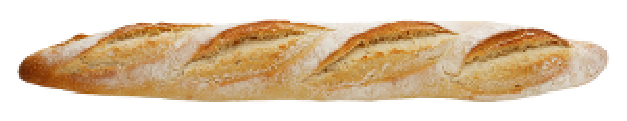
\includegraphics[width=4cm]{Nombres_et_calculs_did/Images/Num4_cours_pain}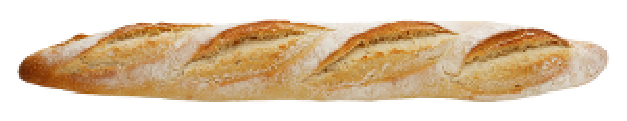
\includegraphics[width=4cm]{Nombres_et_calculs_did/Images/Num4_cours_pain}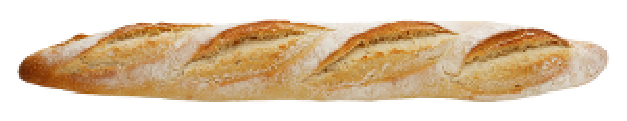
\includegraphics[width=4cm]{Nombres_et_calculs_did/Images/Num4_cours_pain}}
   \psline{|-|}(0,0)(12,0)
   \multido{\n=3+3}{3}{\psline(\n,-3pt)(\n,3pt)}
   \psline[linestyle=dashed](0.02,0)(0.02,-1)
   \psline[linestyle=dashed](3,0)(3,-1)
   \rput(1.5,-0.4){un quart de}
   \rput(1.5,-0.8){trois baguettes}
\end{pspicture}
\end{center}

{\bf $\bullet$ Le fractionnement de l'unité :} ce qui revient à faire \og trois quarts \fg. On partage donc chaque baguette (unité) en quatre parts égales et l'on en prend trois parts.

\begin{center}
\begin{pspicture}(0,-1)(12,1.25)
   \rput(2,0.75){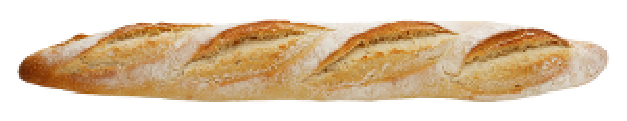
\includegraphics[width=4cm]{Nombres_et_calculs_did/Images/Num4_cours_pain}}
   \psline{|-|}(0,0)(4,0)
   \multido{\n=1+1}{3}{\psline(\n,-3pt)(\n,3pt)}
   \psline[linestyle=dashed](0.02,0)(0.02,-1)
   \psline[linestyle=dashed](3,0)(3,-1)
   \rput(1.5,-0.4){trois quarts}
   \rput(1.5,-0.8){d'une baguette}
\end{pspicture}
\end{center}

Le principe est donc de comprendre que ces deux méthodes mènent à un résultat équivalent, ce que l'on peut écrire de manière mathématique :
$$3\div4 = \dfrac34 =3\times\dfrac14$$

C'est cette équivalence qui fonde le concept de fraction : elle justifie le fait que les deux gestes mentaux précédents soient désignés de la même façon, par la barre de fraction, et que l'on puisse lire indifféremment $3/4$ comme 3 divisé par 4 ou comme trois quarts. \\

{\it Rémi Brissiaud} recommande de commencer par introduire le sens partition de la pluralité (le moins naturel des deux). Sinon, en commençant par le sens le plus naturel, il sera alors difficile d’accéder à l’autre sens. \\

Remarquons que dans notre exemple, le numérateur est inférieur au dénominateur. Le sens \og trois quarts \fg{} est donc prédominant. Supposons maintenant que l'on veuille partager onze baguettes en quatre Dans ce cas, le sens le plus naturel sera certainement de commencer par distribuer deux baguettes à chaque personne, puis à partager les trois baguettes restantes en qutre. \\
On peut dire que \og 11 divisé par 4 est égal à 2 plus le reste, 3, divisé par 4 \fg{} ce qui s'écrit :
$$\dfrac{11}4 =2+\dfrac34.$$


\subsection{Les fractions simples} %%%

D'après ce que nous venons de voir, on peut alors affirmer que les fractions naissent de l’idée de couper une grandeur en parts égales, puis de prélever des parts. Ou que, dans certains cas, une fraction peut aussi exprimer un rapport de deux grandeurs de même nature. \\

Pour les fractions plus petites que l'unité, l'apprentissage des fractions est favorisé par leur représentation sur une bande ou un segment de longueur \og un \fg{} (l'unité de longueur) ou encore grâce à un disque d'aire une unité. \\ [1mm]
Les fractions telles que $\dfrac12, \dfrac14, \dfrac18$ peuvent être facilement illustrées par pliages successifs de l'unité.

\begin{center}
{\psset{unit=0.25}
\begin{pspicture}(-5,-5)(5,5)
   \pscircle[fillstyle=solid,fillcolor=J1](0,0){5}
   \rput(0,0){1}
\end{pspicture}
\qquad
\begin{pspicture}(-5,-5)(5,5)
   \pscircle(0,0){5}
   \pswedge[fillstyle=solid,fillcolor=J1!75](0,0){5}{-90}{90}
   \psline(5;-90)(5;90)
   \rput(3,0){$\dfrac12$}
   \rput(-3,0){$\dfrac12$}
\end{pspicture}
\qquad
\begin{pspicture}(-5,-5)(5,5)
   \pscircle(0,0){5}
   \pswedge[fillstyle=solid,fillcolor=J1!50](0,0){5}{0}{90}
   \psline(5;-90)(5;90)
   \psline(5;0)(5;180)
   \rput(3;45){\small$\dfrac14$}
   \rput(3;135){\small$\dfrac14$}
   \rput(3;-45){\small$\dfrac14$}
   \rput(3;-135){\small$\dfrac14$}
\end{pspicture}
\qquad
\begin{pspicture}(-5,-5)(5,5)
   \pscircle(0,0){5}
   \pswedge[fillstyle=solid,fillcolor=J1!25](0,0){5}{45}{90}
   \psline(5;-90)(5;90)
   \psline(5;0)(5;180)
   \psline(5;-135)(5;45)
   \psline(5;-45)(5;135)
   \rput(3.5;25){\footnotesize$\dfrac18$}
   \rput(3.5;70){\footnotesize$\dfrac18$}
   \rput(3.5;110){\footnotesize$\dfrac18$}
   \rput(3.5;155){\footnotesize$\dfrac18$}
   \rput(3.5;205){\footnotesize$\dfrac18$}
   \rput(3.5;250){\footnotesize$\dfrac18$}
   \rput(3.5;290){\footnotesize$\dfrac18$}
   \rput(3.5;335){\footnotesize$\dfrac18$}
\end{pspicture}}
\end{center}

On peut, à cette occasion, faire le lien avec les grandeurs (capacités, masses, durées). Par exemple, la lecture de l'heure illustre bien ces notions de fractions simples : \\
\begin{center}
{\psset{unit=0.6}
\begin{pspicture}(-2,-2)(8,1.5)
   \pscircle[linewidth=1mm](0,0){2}
   \multido{\i=0+30}{12}{\psline(1.7;\i)(2;\i)} %heures             
   \multido{\i=60+-30,\n=1+1}{12}{\rput(1.5;\i){\footnotesize\n}} %écritures
   \psline[linewidth=0.8mm,linecolor=B2]{->}(0,0)(1;75)
   \psline[linewidth=1mm,linecolor=A1]{->}(0,0)(1.3;-90)
   \psdot(0,0)
   \rput(5,0){midi \og et demi \fg}
\end{pspicture}
\qquad
\begin{pspicture}(-2,-2)(8,1.5)
   \pscircle[linewidth=1mm](0,0){2}
   \multido{\i=0+30}{12}{\psline(1.7;\i)(2;\i)} %heures             
   \multido{\i=60+-30,\n=1+1}{12}{\rput(1.5;\i){\footnotesize\n}} %écritures
   \psline[linewidth=0.8mm,linecolor=B2]{->}(0,0)(1;82.5)
   \psline[linewidth=1mm,linecolor=A1]{->}(0,0)(1.3;0)
   \psdot(0,0)
   \rput(5,0){midi \og et quart \fg}
\end{pspicture}} 
\end{center}

Pour les fractions simples mais plus compliquées à construire, comme $\dfrac13, \dfrac15, \dfrac16$, on peut avoir recours à un réseau de droites parallèles équidistantes aussi appelé \og guide-âne \fg.
\begin{center}
{\psset{yunit=0.9}
\begin{pspicture}(0,-1.5)(12,8.5)
   \psline(0,0)(4,8)
   \psline(1,0)(5,8)
   \psline(2,0)(6,8)
   \psline(3,0)(7,8)
   \psline(4,0)(8,8)
   \psline(5,0)(9,8)
   \psline(6,0)(10,8)
   \psline(7,0)(11,8)
   \psline(8,0)(12,8)
   \psline(9,0)(12,6)
   \psline(10,0)(12,4)
   \psline(11,0)(12,2)
   \psline(3,8)(0,2)
   \psline(0,4)(2,8)
   \psline(0,6)(1,8)
   \psline[linewidth=0.7mm](2,-1)(9,-1)
   \psline[linewidth=0.7mm](0.5,3)(5.8,7.6)
   \psline[linewidth=0.7mm](2,2)(8.4,4.8)
   \psline[linewidth=0.7mm](3.5,1)(10.3,2.6)
   \rput[tl](3.5,-1.2){segment unité de longueur $u$}
   \rput[tl](1.3,4.5){\textcolor{A1}{$\frac13u$}}
   \rput[tl](2.6,3){\textcolor{A1}{$\frac15u$}}
   \rput[tl](4,1.8){\textcolor{A1}{$\frac16u$}}
   \psdots[dotstyle=|,linecolor=B2,linewidth=2mm](2,-1)(9,-1)(0.5,3)(5.8,7.6)(2.3,4.5)(4,6.1)(2,2)(8.4,4.8)(3.3,2.6)(4.6,3.1)(5.8,3.7)(7.1,4.2)(3.5,1)(10.3,2.6)(4.6,1.3)(5.8,1.6)(6.9,1.8)(8,2.1)(9.2,2.4)
\end{pspicture}}
\end{center}
 
À partir du partage de l'unité, on peut passer aux fractions simples dont le numérateur n'est pas 1 : \\ [3mm]
\begin{tabular}{C{8.5}|C{8}}
   {\it Unité de longueur = segment} & {\it Unité de longueur = bande} \\
   \begin{pspicture}(0,-1.5)(8.5,3.5)
      \psline{|-|}(0,0)(3,0)
      \psdots[dotstyle=+](1,0)(2,0)
      \rput[l](3.3,0){\small trois cinquièmes d'unité}
      \psline{|-|}(0,1)(1,1)
      \rput[l](1.3,1){\small un cinquième d'unité}
      \psline{|-|}(0,2)(5,2)
      \psdots[dotstyle=+](1,2)(2,2)(3,2)(4,2)
      \rput[l](5.3,2){\small \parbox{2.8cm}{une unité partagée en cinq parts égales}}
      \psline{|-|}(0,3)(5,3)
      \rput[l](5.3,3){\small une unité}
      \rput[l](0,-1){Fraction représentée : $\dfrac35$}
   \end{pspicture}
   &
   \begin{pspicture}(0,-1.5)(8,3.5)
      \psframe(0,-0.1)(4,0.1)
      \psline(1,-0.1)(1,0.1)
      \psline(2,-0.1)(2,0.1)
      \psline(3,-0.1)(3,0.1)
      \rput[l](4.3,0){\small quatre tiers d'unité}
      \psframe(0,0.9)(1,1.1)
      \rput[l](1.3,1){\small un tiers d'unité}
      \psframe(0,1.9)(3,2.1)
      \psline(1,1.9)(1,2.1)
      \psline(2,1.9)(2,2.1)
      \rput[l](3.3,2){\small \parbox{4cm}{une unité partagée en trois parts égales}}
      \psframe(0,2.9)(3,3.1)
      \rput[l](3.3,3){\small une unité}
      \rput[l](0,-1){Fraction représentée : $\dfrac43$}
   \end{pspicture} \\
\end{tabular}

Le passage du mot à son écriture fractionnaire est une rupture. Jusque-là, pour un élève, un nombre s’écrit avec des chiffres en utilisant le système de numération positionnelle, de gauche à droite. L’écriture d’un nombre sous forme d’une fraction est une nouvelle convention d’écriture dans laquelle les nombres de part et d’autre du trait de fraction ont une signification qu’il convient d’expliciter. Le \og nombre du dessous \fg, appelé dénominateur (celui qui nomme), détermine le nombre de parts en lequel on partage l’unité. C’est celui qui permet de définir la nouvelle unité de comptage. Le \og nombre du dessus \fg, appelé numérateur (celui qui compte), détermine le nombre d’unités de comptage que l’on considère.

Les fractions supérieures à 1 doivent très vite être abordées, car les élèves ont l'habitude d'utiliser les fractions comme des \og morceaux de \fg, et des fractions telles que $\dfrac83$ par exemple n'ont pas toujours du sens pour les élèves. \\
Pour expliciter la compréhension d'une telle fraction, on peut écrire la fraction sous forme de somme d'un entier et d'une fraction inférieure à 1.  Cette écriture permet d'obtenir un ordre de grandeur du nombre représenté par cette fraction et d'encadrer facilement la fraction par deux nombres entiers consécutifs.

\begin{pspicture}(-2.5,-1.5)(1,1.5)
   \pscircle[fillstyle=solid,fillcolor=J1](0,0){1} 
   \psline(0,0)(1;-30)
   \psline(0,0)(1;90)
   \psline(0,0)(1;-150)
\end{pspicture}
\begin{pspicture}(-1.5,-1.5)(1,1.25)
   \SpecialCoor
   \pscircle[fillstyle=solid,fillcolor=J1](0,0){1}
   \psline(0,0)(1;-30)
   \psline(0,0)(1;90)
   \psline(0,0)(1;-150)
\end{pspicture}
\begin{pspicture}(-1.5,-1.5)(1,1.25)
   \SpecialCoor   
   \pscircle(0,0){1}
   \pswedge[fillstyle=solid,fillcolor=J1!50](0,0){1}{210}{90}
   \psline(0,0)(1;-30)
   \rput(5,0){$\dfrac83 =2+\dfrac23$ donc, $\dfrac83$ est compris entre 2 et 3.}
\end{pspicture}

Les nombres, exprimés sous forme de fractions simples, permettent aussi de repérer un point sur une demi-droite graduée. Pour cela, on partage l’unité en parts égales correspondant au dénominateur de la fraction, on reporte ensuite la fraction autant de fois que nécessaire. L’écriture d’une fraction comme somme d’un entier et d’une fraction comprise entre 0 et 1 est particulièrement utile pour placer une fraction sur une droite graduée et donne du sens au travail mené pour passer d’une écriture à l’autre.

\begin{pspicture}(0,0)(16.5,3)
   \psframe(0,2)(4,2.5)%1
   \rput(2,2.25){\small1 unité}
   \psframe(4,2)(8,2.5)
   \rput(6,2.25){\small1 unité}
   \psframe(8,2)(12,2.5)
   \rput(10,2.25){\small1 unité}
   \psframe(12,2)(16,2.5)
   \rput(14,2.25){\small1 unité}
   \psframe(0,1)(4,1.5)%2
   \rput(2,1.25){\small1 unité}
   \psframe(4,1)(8,1.5)
   \rput(6,1.25){\small1 unité}
   \psframe(8,1)(9.33,1.5)
   \rput(8.67,1.25){$\frac13$}
   \psframe(9.33,1)(10.67,1.5)
   \rput(10,1.25){$\frac13$}
   \psaxes[dx=4,yAxis=false](0,0.25)(16.5,0.25)%3
   \rput(10.67,0.25){|}
   \rput(9.33,0.25){|}
   \rput(10.66,-0.2){$\frac83$}
\end{pspicture} \\


\subsection{Les fractions décimales} %%%

Le travail sur les fractions simples conduit à rencontrer des fractions ayant un dénominateur égal à 10. Il prépare l’introduction des fractions décimales, définies comme des fractions particulières correspondant à un partage de l’unité en 10, 100 ou 1 000 à l'école. Il faut prendre l'habitude de lire les fractions de la manière suivante afin d'anticiper le travail sur les nombres décimaux : 
$\dfrac1{10}$ se lit \og un dixième \fg, $\dfrac1{100}$ \og un centième \fg, $\dfrac1{1\,000}$ \og un millième \fg.

    Par continuité avec les pliages en 2, 3, 4\dots{} on fait au moins une fois avec les élèves le pliage en 10 même si ce n'est pas simple. 
    \begin{center}
       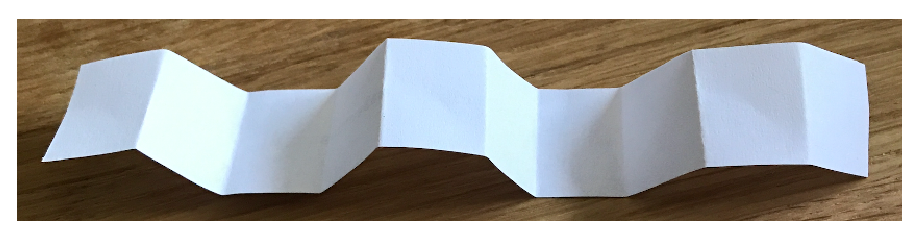
\includegraphics[width=10cm]{Nombres_et_calculs_did/Images/Num4_cours_bande_dixieme}
    \end{center}
    L'intérêt est de montrer l'aspect récursif de la méthode : après avoir partagé en 10, on peut encore partager chaque dixième en 10\dots \\
    Le fait que 10 dixièmes soit égal à une unité, que 10 centièmes soit égal à 1 dixième et que 100 centièmes soit égal à 1 unité doit être explicité par l'utilisation de matériel permettant la manipulation et la visualisation de ces partages. \\
    Un grand carré unité divisé en 100 petits carrés permet un type de modélisation. \\
    \begin{minipage}{8cm}
       \begin{center}
       \psset{unit=0.5}
          \begin{pspicture}(0,-1)(10,11)
             \psgrid[subgriddiv=0,gridlabels=0,gridcolor=B1](0,0)(10,10)
             \psset{,linewidth=0.5mm}
             \psframe(0,0)(10,10)
             \multido{\n=1+1}{9}{\psline(0,\n)(10,\n)}
          \end{pspicture}
       \end{center}
    \end{minipage}
    \begin{minipage}{8cm}
       On a les représentations suivantes : \\ [2mm]
       $\bullet$ il y a 100 petites carrés dans le grand carré donc, un petit carré représente 1 centième de l'unité, soit $\dfrac{1}{100}$. \\ [2mm]
       $\bullet$ il y a 10 lignes dans le grand carré donc, une ligne représente 1 dixième de l'unité, soit $\dfrac{1}{10}$. \\ [2mm]
       $\bullet$ il y a 10 petites carrés dans une ligne donc, 10 centièmes valent 1 dixième.
    \end{minipage}

    La bande unité, quant à elle, permet de représenter les valeurs des fractions décimales de manière plus linéaire.
    \begin{center}
       \begin{pspicture}(0,-0.8)(16,1)
          \multido{\n=0.16+0.16}{99}{\psline[linecolor=B1](\n,0)(\n,0.5)}
          \psframe(0,0)(16,1)
          \multido{\n=1.6+1.6}{9}{\psline(\n,0)(\n,1)}
          \rput(0,-0.5){0}
          \rput(16,-0.5){1}
          \multido{\n=1.6+1.6,\i=1+1}{9}{\rput(\n,-0.5){$\frac{\i}{10}$}}
          \psline[linecolor=B1]{->}(0.16,-0.1)(0.16,-0.7)
          \rput(0.16,-1){\textcolor{B1}{$\frac{1}{100}$}}
       \end{pspicture}
    \end{center}

Le travail sur les relations entre les différentes unités de numération permet de faire le lien entre différentes écritures d’un même nombre décimal dont deux seront particulièrement mises en avant : \\ [1mm]
$\bullet \; \dfrac{753}{100} =7+\dfrac{53}{100}$. Cette écriture correspond à la décomposition du nombre décimal en la somme de sa partie entière\\[1mm]et de sa partie décimale. Elle est utile pour les calculs, les comparaisons et le repérage sur une droite graduée. \\ [2mm]
$\bullet \; \dfrac{753}{100} =7+\dfrac{5}{10}+\dfrac{3}{100}$ est la somme d'un entier et de fractions décimales  de dénominateurs différents. Cette écriture\\[1mm]prépare l’introduction de l’écriture à virgule des nombres décimaux.


%%%%%%%%%%%%%%%%
\section{Les nombres décimaux}
%%%%%%%%%%%%%%%%

\subsection{La construction des décimaux} %%%

   Au cycle 3, les nombres décimaux sont introduits à partir des fractions décimales. L’écriture à virgule est présentée comme une convention d’écriture d’une fraction décimale ou d’une somme de fractions décimales (codage). Cette notation permet la mise en place des règles de comparaison et de calcul. \\ [1mm]
   Par exemple, le nombre $\dfrac{16\,802}{1\,000}=16+\dfrac{8}{10}+\dfrac{0}{100}+\dfrac{2}{1\,000} =16+\dfrac{802}{1\,000}$ peut s'écrire \\ [2mm]
   \begin{tabular}{cccccccc}
        $\dfrac{16\,802}{1\,000}$ & = &$1\times10$ + & $6\times 1$ + & & $8\times \dfrac{1}{10}$ + & $0\times \dfrac{1}{100}$ + & $2\times \dfrac{1}{1000}$ \\ [3mm]
       & = & 1 & 6 & , & 8 & 0 & 2 \\ [1mm]
       & & \rotatebox{60}{\footnotesize chiffre des dizaines} & \rotatebox{60}{\footnotesize chiffre des unités} & & \rotatebox{60}{\footnotesize chiffre des dixièmes} & \rotatebox{60}{\footnotesize chiffre des centièmes} & \rotatebox{60}{\footnotesize chiffre des millièmes} \\
   \end{tabular}

\smallskip

Pour la partie fractionnaire, on utilise le vocabulaire \og{}dixième\fg{}, \og{}centième\fg{}, \og{}millième\fg{} en articulant correctement afin de ne pas confondre avec \og{}dizaine\fg{}, \og{}centaine\fg{}, \og{}millier\fg. Dans un premier temps, il faudra faire attention à bien \og dire \fg{} les nombres décimaux : on ne dit pas \og{}seize virgule huit-cent-deux \fg{} mais \og{} seize et huit-cent-deux millièmes \fg{} ou \og{}seize, huit dixièmes et deux millièmes \fg. \\
   On peut profiter de l'occasion pour faire le parallèle avec le tableau de numération, que l'on prolonge vers la droite.
\begin{center}
\begin{Ltableau}{0.9\linewidth}{9}{c}
   \hline
   \multicolumn{5}{|c@{\bf , }}{\bf partie entière} & \multicolumn{4}{c|}{\bf partie décimale} \\
   \hline
   \ldots & milliers & centaines & dizaines & unités & dixièmes & centièmes & millièmes & \ldots \\
   \hline
   & & & 1 & 6 & 8 & 0 & 2 & \\
   \hline
\end{Ltableau}
\end{center}  
La comparaison de deux nombres décimaux se fait alors ordre par ordre : 2,5 est plus grand que 2,46 car ils ont la même partie entière, mais 2,5 comporte 5 dixièmes alors que 2,46 n'en comporte que 4\dots{} cela suffit pour conclure ! On évitera d'employer la \og recette de cuisine \fg{} consistant à ajouter des \og 0 \fg{} à l'un des nombres jusqu'à obtenir le même nombres de chiffres après la virgule puis comparer leur partie décimale : en effet, c'est procédure renforcerait l'idée que l'on pourrait comparer les parties décimales comme s'il s'agissait de nombres entiers.

L’utilisation régulière de la demi-droite graduée, avec d’éventuels zooms successifs, permet de travailler l’intercalation entre deux décimaux et de déterminer la position d’un nombre sur la demi-droite graduée avec de plus en plus de précision. Cela contribuera également à aider les élèves à ne pas voir un nombre décimal comme deux entiers séparés par une virgule, mais bien comme un nombre à part entière.

{\psset{unit=0.85}
\begin{pspicture}(-4,-4)(12,1.3)
   \mili{0}{1}{12}{-5}
   \rput(1,0){
   \multido{\n=0+1,\i=0+1}{11}{\psline[linewidth=1pt](\i,-.1)(\i,.1) \uput[d](\i,0){\footnotesize \n}}
   \psline{->}(0,0)(10.5,0)}
   \rput(1,-2){\multido{\n=3.0+.1,\i=0+1}{11}{\psline[linewidth=1pt](\i,-.1)(\i,.1) \uput[d](\i,0){\footnotesize \n}}
   \psline{->}(0,0)(10.5,0)}
   \rput(1,-4){\multido{\n=3.10+.01,\i=0+1}{11}{\psline[linewidth=1pt](\i,-.1)(\i,.1) \uput[d](\i,0){\footnotesize \n}}
   \psline{->}(0,0)(10.5,0)}
   \psset{linewidth=1pt,linecolor=B2,linestyle=dashed}
   \psline(4,0)(1,-2)
   \psline(2,-2)(1,-4)
   \psline(5,0)(11,-2)
   \psline(3,-2)(11,-4)
\end{pspicture}}


\subsection{Les erreurs liées aux nombres décimaux} %%%

L'enseignant.e doit faire attention à ne pas nommer un nombre décimal comme s'il s'agissait d'un couple de nombres entiers : c'est en effet l'erreur la plus fréquente chez l'élève. De plus, les propriétés de la structure de l'ensemble des nombres entiers utilisée jusque là ne se généralisent pas au niveau des nombres décimaux.
\begin{center}
{\renewcommand{\arraystretch}{1.2}
\begin{Ltableau}{1\linewidth}{2}{p{8cm}|p{8cm}}
   \hline
   Nombres entiers & Nombres décimaux \\
   \hline
   Tout nombre entier a un prédécesseur (sauf 0) et un successeur. & Le prédécesseur ou le successeur d'un nombre décimal n'a aucun sens. \\
   $\bullet$ {\it Le prédécesseur de 4 est 3, son successeur est 5.} & $\bullet$ {\it Quel serait le successeur de 4 ? de 5,7 ?} \\
   \hline
   Entre deux nombres entiers consécutifs, il n'y a pas de nombre entier. & Entre deux nombres décimaux consécutifs, il n'y a une infinité de nombre décimaux. \\
   $\bullet$ {\it Entre 12 et 13, il y a aucun entier} & $\bullet$ {\it Entre 13 et 14, on a par exemple 13, 5 ou 13,68\dots} \\
   \hline
   Entre deux nombres entiers, il y a un nombre fini de nombres entiers. & Entre deux nombres décimaux, il y a une infinité de nombres décimaux. \\
   $\bullet$ {\it Entre 5 et 8, il n'y a 6 et 7 uniquement.} & $\bullet$ {\it Entre 5 et 8, on a par exemple 5,6 ou 7 ou 7,999\dots} \\
   \hline
   Plus un nombre entier a de chiffres, plus il est grand. & Le nombre de chiffres d'un nombre décimal n'a aucune incidence sur sa grandeur. \\
   $\bullet$ 1\,234 est plus grand que 123. & $\bullet$ 1,235 est plus petit que 12,4. \\
   \hline  
   Un nombre entier était jusque là représenté sur une frise numérique. & On représente dorénavant les nombres décimaux (y compris les entiers) sur une droite graduée. \\
   \hline
\end{Ltableau}}
\end{center}

Autres conceptions erronées des élèves :
\begin{center}
{\renewcommand{\arraystretch}{1.2}
\begin{Ltableau}{1\linewidth}{2}{p{8cm}|p{8cm}}
   \hline
   Erreurs et difficultés & Exemples \\
   \hline
   Assimilation de la virgule à un trait de fraction & $\dfrac35 =3,5$. \\ [2mm] 
   \hline
   Difficulté à concevoir qu’un même nombre puisse avoir plusieurs désignations. &
   $\bullet$ {\it $1+\dfrac{4}{10} =1,4 =1,40$ sont perçus comme des nombres différents.} \\
   \hline
   Nombre à virgule vu comme deux entiers séparés par une virgule. &
   {\it $\bullet$ $4,3 < 4,26 < 4,249$ car $3 < 26 < 249$. \newline
   $\bullet$ 2,47 est le successeur de 2,46. \newline
   $\bullet$ $2,3+7,12=9,15$ puisque $2+7=9$ et $3+12 =15$.} \\
   \hline
   Connaissance mal installée du système décimal. &
   {\it $\bullet$ Dans 12,345 le chiffre centièmes est 3 puisque 3 est le chiffre des centaines dans 345. \newline
   $\bullet$ Dans $234,678$ le chiffre des dixièmes est 7 en raison de la position supposée des dixièmes comme symétrique de celle des dizaines. \newline
   $\bullet$ $4,249 < 4,16 < 4,1$ puisque  les millièmes sont forcément plus petits que les centièmes, eux-mêmes plus petits que les dixièmes.} \\
   \hline
   Application de règles au-delà de leur domaine de validité. &
   {\it $\bullet$ $1,4\times10 = 1,40$ ou 10,4 puisqu'on ajoute un \og 0 \fg{} à la fin de l'écriture du nombre.} \\
   \hline
   Usage social des nombres décimaux à l’oral à l’origine de confusions. &
   {\it $\bullet$ Un kilo cinq s’écrit 1,5 kg alors que un euro cinq s’écrit 1,05 euros.} \\
   \hline
\end{Ltableau}}
\end{center}


%%%%%%%%%%%%%%%%%%%%%%%%%%%%%
%%%%%%%%%%%%%%%%%%%%%%%%%%%%%
\activites

\textcolor{G1}{Sujet n°6 de l'épreuve de leçon, concours CRPE 2022, académie de Montpellier.} \bigskip

{\bf\uline{Consigne candidat}} : À partir du sujet et du dossier proposés par le jury, vous concevrez la mise en œuvre d'une séance d'enseignement à l'école primaire dans chacune des deux disciplines français et mathématiques. Vous présenterez successivement les composantes pédagogiques et didactiques de chaque séance et son déroulement. \medskip

{\bf\uline{Sujet}} : Introduction de la notion de fraction. \medskip

{\bf\uline{Contexte de la séance d'enseignement}} : \\
   \hspace*{5mm} -- cycle d'enseignement : cycle 3 ; \\
   \hspace*{5mm} -- niveau de la classe : CM1 ; \\
   \hspace*{5mm} -- positionnement de la séance de mathématiques : \\
      \hspace*{10mm} -- période : période 1 ou 2 ; \\
      \hspace*{10mm} -- séquence dans laquelle elle s'insère : utiliser et représenter des fractions simples. \bigskip

{\bf\uline{Documents fournis au candidat}} : \medskip

{\bf\uline{Document 1}} : Document Éduscol d'après le BOEN n°31 du 20 juillet 2020, {\it Programme du cycle 3 en vigueur à la rentrée 2020}, extrait de la page 93.

\begin{center}
   \textsf{
      \begin{tabular}{p{15cm}}
         \cellcolor{A3!50}{{\bf Attendus de fin de cycle} \newline
         -- Utiliser et représenter les grands nombres entiers, des fractions simples, les nombres décimaux. \newline
         -- Calculer avec des nombres entiers et des nombres décimaux. \newline
         -- Résoudre des problèmes en utilisant des fractions simples, les nombres décimaux et le calcul.} \\
      \end{tabular}
   }
   
   \medskip
   
   \textsf{
      \begin{tabular}{|p{14.9cm}|}
         \hline
         \textcolor{teal}{\bf Utiliser et représenter les grands nombres entiers, des fractions simples, les nombres décimaux} \\
         \hline
         Connaître diverses désignations des fractions : orales, écrites et décompositions additives et multiplicatives (ex : quatre tiers ; 4/3 ; 1/3 + 1/3 + 1/3 + 1/3 ; 1 + 1/3 ; 4 $\times$ 1/3). \newline
         Connaître et utiliser quelques fractions simples comme opérateur de partage en faisant le lien entre les formulations en langage courant et leur écriture mathématique (ex : faire le lien entre \og la moitié de \fg{} et multiplier par 1/2). \newline
         Utiliser des fractions pour rendre compte de partages de grandeurs ou de mesures de grandeurs. Repérer et placer des fractions sur une demi-droite graduée adaptée. \newline
         Encadrer une fraction par deux nombres entiers consécutifs. Comparer deux fractions de même dénominateur. \newline
         Écrire une fraction sous forme de somme d’un entier et d’une fraction inférieure à 1. Connaître des égalités entre des fractions usuelles (ex : 5/10 = 1/2 ; 10/100 = 1/10 ; 2/4 = 1/2). Utiliser des fractions pour exprimer un quotient. \\
         \hline
   \end{tabular}
   }
\end{center}

\medskip


{\bf\uline{Document 2}} : Image tirée de \og Séquence sur les fractions et les décimaux \fg, séquence tirée de ERMEL, retravaillée par le groupe 1\up{er} degré de I'IREM de Montpellier au cours de l'année scolaire 201612017, et prise dans une classe de CM1-CM2 de l'école J. Rostand de Clermont I'Hérault.

\begin{center}
   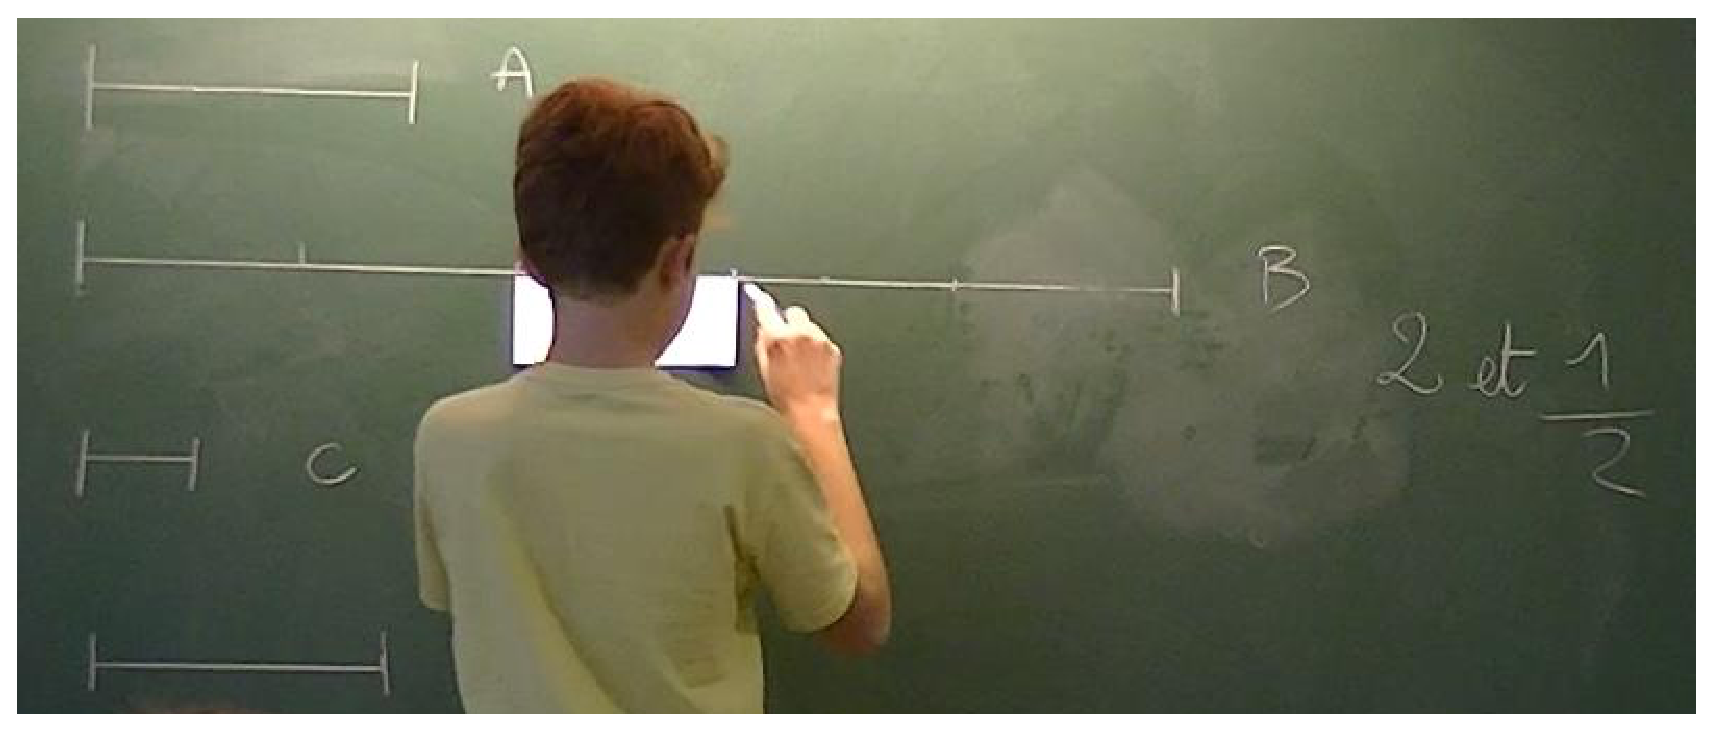
\includegraphics[width=10cm]{Nombres_et_calculs_did/Images/Num4_crpe_fractions_IREM}
\end{center}


{\bf\uline{Document 3}} : R. Charnay, B. Anselmo, G. Combiet, M.P. Dussuc, D. Madier, M. Front, A. Ravoux, \og Fractions simples \fg, {\it Nouveaux CAP MA THS CM1}, Paris, Éditions Hatier, 2020, page 30.

\begin{center}
   \fbox{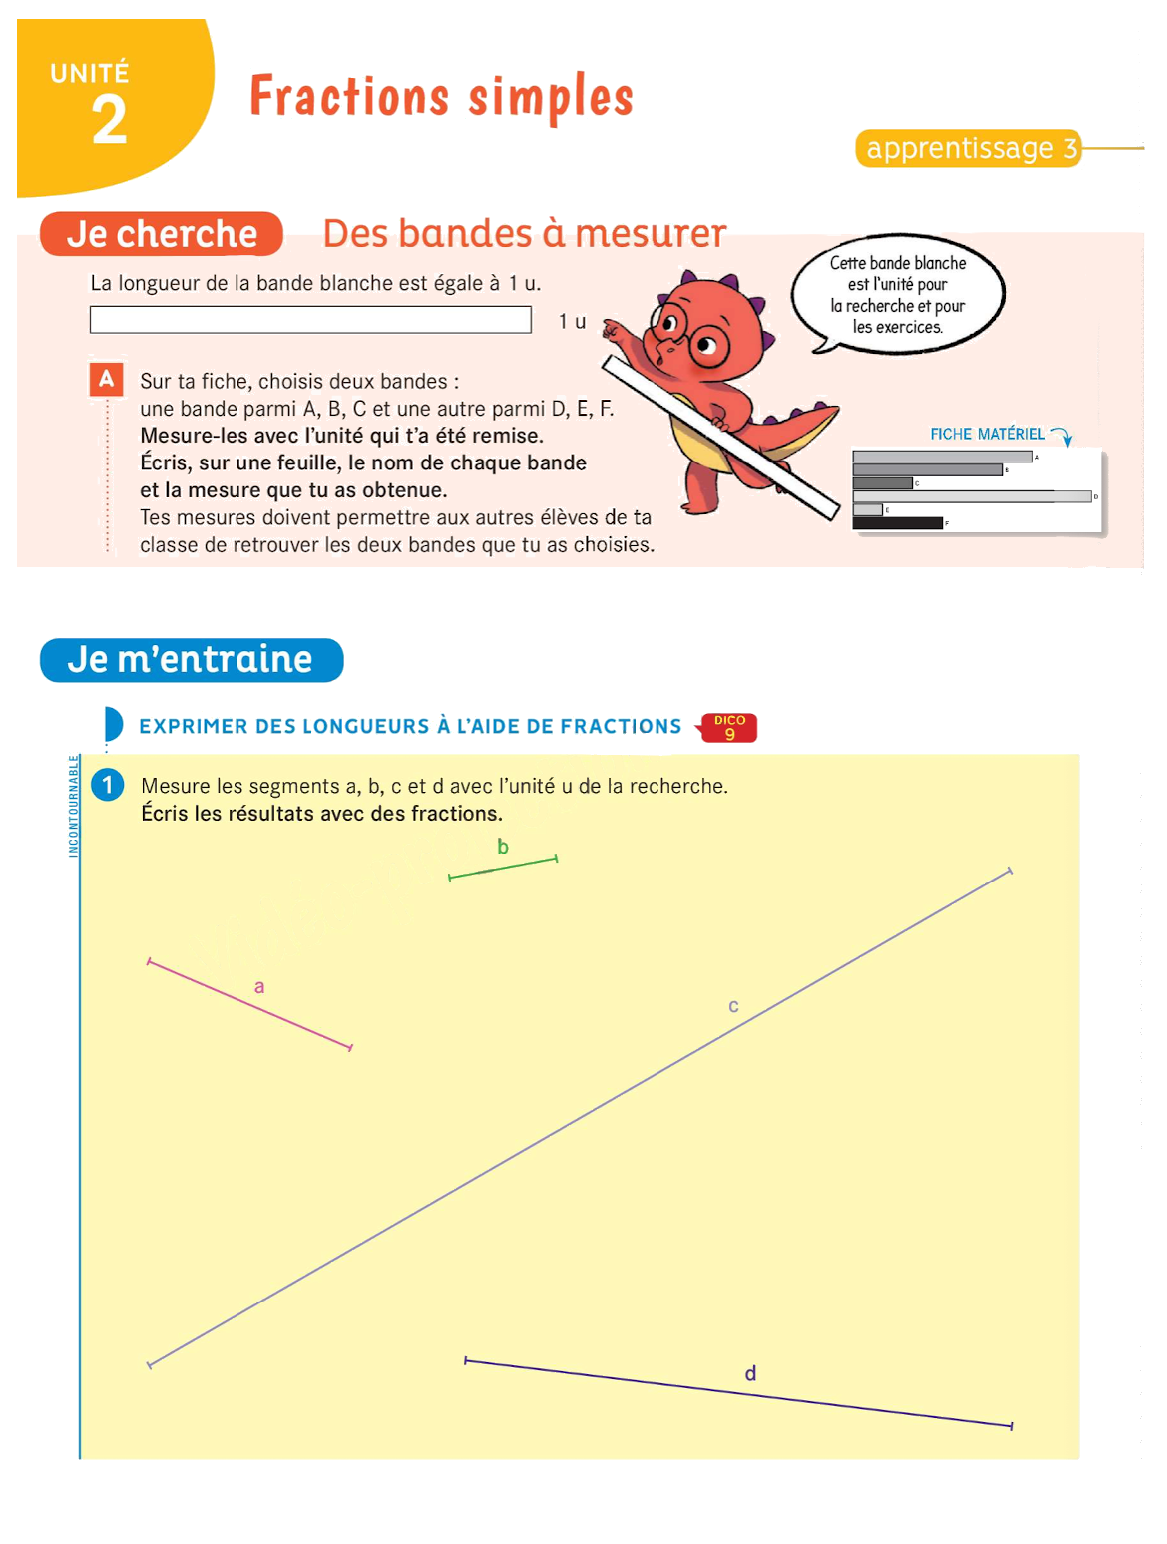
\includegraphics[width=15.5cm]{Nombres_et_calculs_did/Images/Num4_crpe_fractions_CM}}
\end{center}


{\bf\uline{Document 4}} : Hélène Zucchetta et Bernard Anselmo, {\it Construire les nouveaux nombres au cycle 3. Fractions et décimaux}, Canopé éditions, Mars 2018, extrait de la page 145.

\begin{center}
   \textsf{\small
      \begin{pspicture}(0,0.4)(15.2,21.4)
         \psframe(0,0)(15.2,21.4)
         \rput{90}(1,11){Coller ici une unité entière non pliée}
         \rput[l](1,20.7){\underline{SITUATION 1 - ANNEXE 4 - ÉLÈVE}}
         \rput[r](14,20.7){\underline{CANOPÉ / IREM DE LYON}}
         \rput[l](2.6,19.3){\bf\large Des nouveaux nombres pour mesurer}
         \rput[l](2.6,18.4){Les nombres entiers ne suffisent pas toujours pour \makebox[3.5cm]{\dotfill}}
         \rput[l](2.6,17.9){Il est parfois nécessaire de partager \makebox[3.5cm]{\dotfill}}
         \rput[l](2.6,17.4){On utilise alors des \makebox[3.1cm]{\dotfill}}
         \rput[l](2.6,16.1){\bf 1. Partage de l'unité}
         \rput[l](2.6,15.5){a) En 2 parties égales.}
         \rput[l](5.7,15.5){Les parties obtenues s'appellent}
         \multido{\r=15.5+-0.5}{5}{\rput[l](9.5,\r){\makebox[3.5cm]{\dotfill}}}
         \rput[l](2.6,12.5){b) En 4 parties égales.}
         \rput[l](5.7,12.5){Les parties obtenues s'appellent}
         \multido{\r=12.5+-0.5}{5}{\rput[l](9.5,\r){\makebox[3.5cm]{\dotfill}}}
         \rput[l](2.6,9.5){c) En 8 parties égales.}
         \rput[l](5.7,9.5){Les parties obtenues s'appellent}
         \multido{\r=9.5+-0.5}{5}{\rput[l](9.5,\r){\makebox[3.5cm]{\dotfill}}}  
         \rput[l](2.6,6.2){\bf 2. Explication des écritures}    
         \rput[l](2.6,5.6){$\frac12u$, c'est l'unité partagée en \makebox[1cm]{\dotfill} parties égales et je prends \makebox[1cm]{\dotfill} de ces parties.}
         \rput[l](2.6,4.9){$\frac34u$, c'est l'unité partagée en \makebox[1cm]{\dotfill} parties égales et je prends \makebox[1cm]{\dotfill} de ces parties.} 
         \rput[l](2.6,4.2){$\frac38u$, c'est l'unité partagée en \makebox[1cm]{\dotfill} parties égales et je prends \makebox[1cm]{\dotfill} de ces parties.}   
         \rput[l](2.6,3.5){$\frac88u$, c'est 8 fois \makebox[2cm]{\dotfill} d'unité.} 
         \rput[l](2.6,2.8){Dans l'écriture $\frac38u$, 8 est le \makebox[3cm]{\dotfill} et 3 est le  \makebox[3cm]{\dotfill}.}
         \rput[l]{90}(13.4,1){Tracer ici un segment mesurant $\frac34$ d'unités puis donner d'autres écritures de $\frac34$ d'unités}
         \psline{|-}(13.7,1)(13.7,20.3)
         \rput[l]{90}(14.2,1){Tracer ici un segment mesurant $\frac88$ d'unités puis donner d'autres écritures de $\frac88$ d'unités}
         \psline{|-}(14.5,1)(14.5,20.3)
      \end{pspicture}
   }
\end{center}


%%%%%%%%%%%%%%%%%%%%%%%%%%%%
%%%%%%%%%%%%%%%%%%%%%%%%%%%%
\analyses

%\begin{exercice*}[CRPE 2003 Grenoble]
%   Les extraits suivants présentent quatre productions d'élèves obtenues dans le cadre de l'évaluation nationale effectuée en 6\up{ème} à la rentrée scolaire de septembre 2002. \\
%   Les élèves devaient répondre, en temps limité, dans la partie gauche du document, sans autre instruction que ce qui est écrit. \\  
%   Le correcteur a entouré, dans la partie droite, le code à un chiffre (entre 0 et 9) qui traduit la réponse de l'élève, selon les consignes de codage fournies par le ministère.
%   \begin{itemize}
%      \item 1 : réponse exacte attendue, procédure induite par l'énoncé, objectif atteint ;
%      \item 2 : réponse exacte, formulation moins attendue ou non exhaustive, mais on considère que l'objectif est atteint par l'élève ;
%      \item 5 : réponse pouvant être interprétée comme une mauvaise lecture de consigne ;
%      \item 6 et 7 : réponse erronée spécifiée ;
%      \item 9 : autre réponse erronée ;
%      \item 0 : absence de réponse.
%   \end{itemize}
%   \vspace*{-5mm}
%\begin{enumerate}
%   \item Pour l'élève Enzo, dans l'exercice 12, le code 5 a été retenu.
%   \begin{enumerate}
%      \item Quelle erreur a-t-il commise ?
%      \item Proposez deux hypothèses qui peuvent expliquer cette erreur.
%      \item Comment expliquer alors sa réussite à l'exercice 13 ?
%\end{enumerate}
%   \item Les réponses des élèves Nadia et Thomas dans l'exercice 12 sont codées 7.
%   \begin{enumerate}
%      \item Quelle est leur erreur commune dans le traitement des nombres ?
%      \item Quel obstacle dans l'apprentissage des nombres peut être à l'origine de cette erreur ?
%   \end{enumerate}
%   \item Dans l'exercice 13, on a constaté, au niveau national, que :
%   \begin{itemize}
%      \item seulement 57,6\% des élèves ont donné une réponse juste,
%      \item 27,4\% des élèves ont commis la même erreur qu'Aude et Thomas.
%   \end{itemize}
%   \vspace*{-5mm}
%   \begin{enumerate}
%      \item Donnez deux raisons qui expliquent le faible taux de réussite à cet exercice.
%      \item Pourquoi l'erreur commise par Aude et Thomas est-elle si fréquente ?
%   \end{enumerate}
%\end{enumerate}
%\begin{center}
%   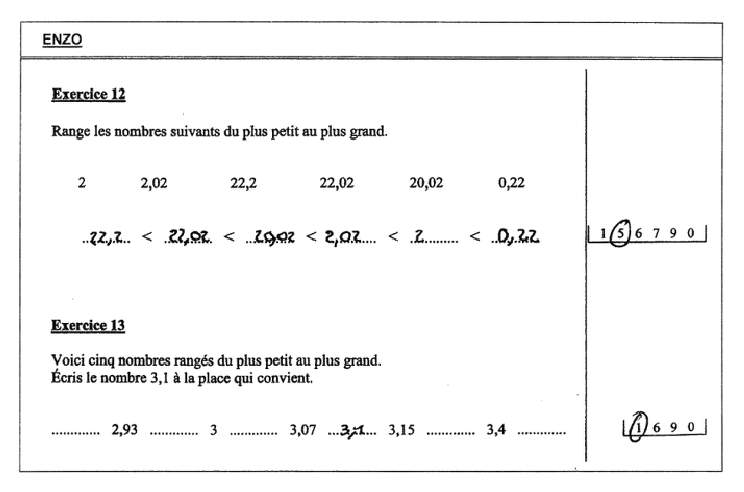
\includegraphics[width=11.25cm]{Nombres_et_calculs_did/Images/Num4_analyse_Enzo} \\
%   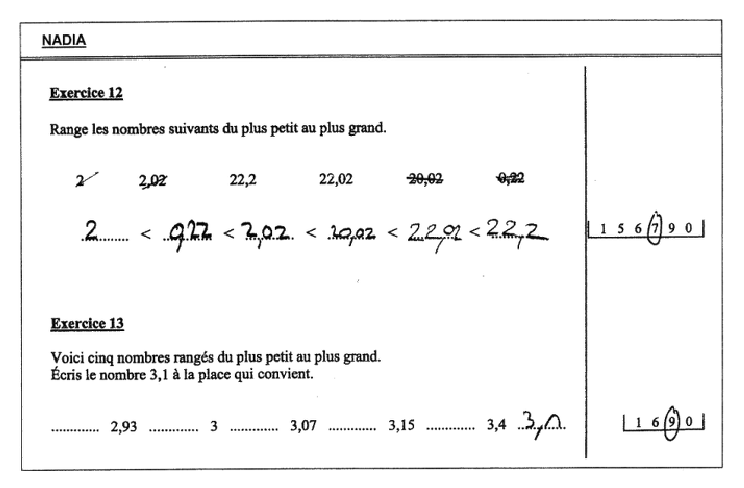
\includegraphics[width=11.25cm]{Nombres_et_calculs_did/Images/Num4_analyse_Nadia} \\   
%   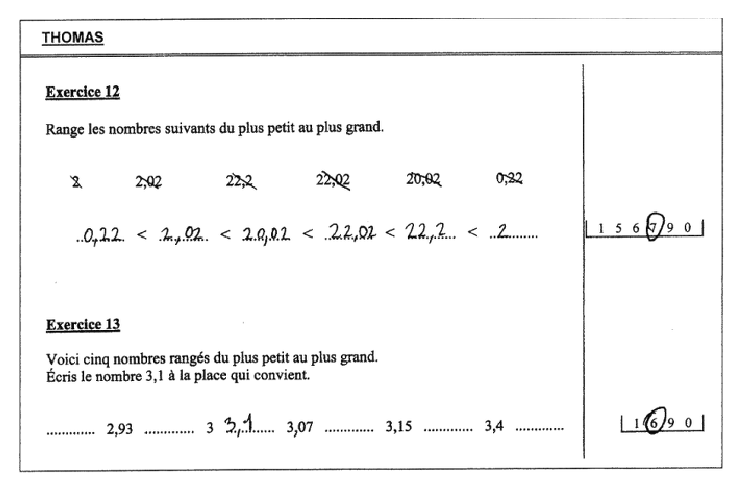
\includegraphics[width=11.25cm]{Nombres_et_calculs_did/Images/Num4_analyse_Thomas} \\  
%   \includegraphics[width=11.25cm]{Nombres_et_calculs_did/Images/Num4_analyse_Aude}
%\end{center}
%\end{exercice*}
%
%\begin{corrige}
%\ \\ [-5mm]
%\begin{enumerate}
%   \item
%   \begin{enumerate}
%      \item Enzo range dans l'ordre inverse de celui demandé. Il maîtrise donc l'ordre des nombres, mais ne respecte pas la consigne.
%      \item \textcolor{A2}{$\bullet$} il confond les symboles \og > \fg{} et \og < \fg. 
%      \begin{itemize}
%         \item il interprète mal la consigne du plus petit au plus grand en inversant le sens ;
%      \end{itemize}
%      \item Ici il n' y a pas à interpréter la consigne du plus petit au plus grand car les cinq nombres donnés sont déjà placés, étant donné qu'Enzo semble maitriser l'ordre des nombres, ainsi que les nombres décimaux, il lui reste juste à insérer 3,1 à la bonne place.
%   \end{enumerate}
%   \item
%   \begin{enumerate}
%      \item Les nombres décimaux non entiers sont bien rangés entre eux, mais Nadia et Thomas placent mal le nombre entier : en premier pour Nadia, à la fin pour Thomas.
%      \item Ils ne considèrent sans doute pas les entiers comme des décimaux particuliers. Ils rangent donc les entiers, puis les décimaux ou inversement comme s'ils faisaient un tri.
%   \end{enumerate}
%   \item
%   \begin{enumerate}
%      \item Raisons probables : 
%      \begin{itemize}
%         \item les nombres ont une écriture différente avec une partie décimale comportant entre 0 et 2 chiffres ;
%         \item 3,1 a un chiffre après la virgule et il doit être placé entre deux nombres à deux chiffres après la virgule ;
%         \item les nombres placés sont ordonnés du plus petit au plus grand. 3,1 va donc être placé \og juste après \fg{} 3.
%      \end{itemize}
%      \item L'erreur est fréquente car elle peut être la conséquence de plusieurs théorèmes en acte des élèves : 
%      \begin{itemize}
%         \item un nombre décimal est considéré comme deux entiers séparés par une virgule, donc : 3,1 <  3,07 car 1 < 7 ;    
%         \item 3,1 est considéré comme le successeur de 3 ;
%         \item les décimaux sont traités comme des entiers (on ne s'occupe pas de la virgule). On a alors 3 < 31 < 307.
%   \end{itemize}
%   \end{enumerate}
%\end{enumerate}
%\end{corrige}
%
%\bigskip

\begin{exercice}[CRPE 2014 G1]
{\bf A.} En classe de CM1, un enseignant propose en application de la leçon sur les nombres décimaux les deux exercices suivants :
\begin{center}
\fbox{\begin{minipage}{15cm}
   {\bf Exercice 1} \\
   Calcule les sommes suivantes : \qquad $0,3 + 0,8$ \qquad $1,3 + 0,12$
\end{minipage}}
\end{center}
\begin{center}
\fbox{\begin{minipage}{15cm}
   {\bf Exercice 2} \\
   Range dans l'ordre croissant les nombres décimaux suivants : \\
   \hspace*{2cm} $5,100$ \qquad $5,6$ \qquad $5,03$
\end{minipage}}
\end{center}
\begin{enumerate}
   \item Voici les réponses d'un élève à l'exercice 1 :
   \begin{center}
   \fbox{\begin{minipage}{5cm}
      $0,3+0,8= 0,11$ \\
      $1,3+0,12= 1,15$
   \end{minipage}}
   \end{center}
   À partir de ces réponses, indiquer ce que cet élève semble maîtriser et ce qu'il lui reste à travailler.
   \item Voici la réponse d'un élève à l'exercice 2 :
   \begin{center}
   \fbox{\begin{minipage}{5cm}
      $5,03 < 5,6 < 5,100$
   \end{minipage}}
   \end{center}
   \begin{enumerate}
      \item Quelle représentation erronée des nombres décimaux pourrait être à l'origine de l'erreur de cet élève ? Justifier.
      \item Quelle désignation orale des nombres 5,03 ; 5,6 et 5,100 l'enseignant pourrait-il utiliser pour aider les élèves à se construire une bonne représentation des nombres décimaux ?
   \end{enumerate}
\end{enumerate}

\textbf{B.} En classe de CM2, un autre enseignant propose l'exercice de réinvestissement suivant :
\begin{center}
   \fbox{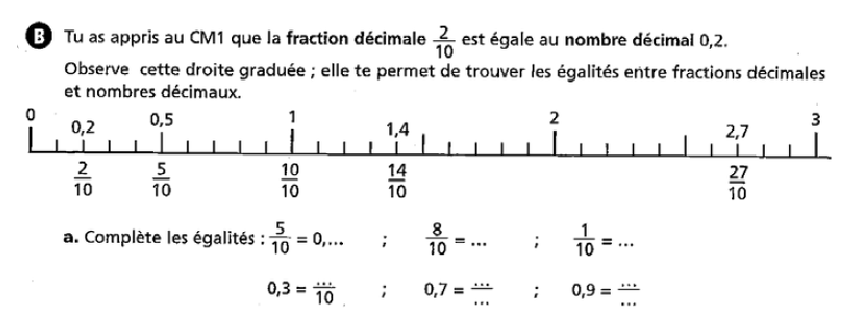
\includegraphics[width=14cm]{Nombres_et_calculs_did/Images/Num4_analyse_droite_graduee}} \\
   {\it Extrait du manuel \og Pour comprendre les mathématiques CM2 \fg, Hachette 2005.}
\end{center}
\begin{enumerate}
   \item Quelle définition d'un nombre décimal peut-on donner à l'école élémentaire ?
   \item Un élève affirme que la somme de deux nombres décimaux ne pourra jamais être un nombre entier. Comment l'enseignant peut-il utiliser le support de l'exercice {\bf B} pour lui apporter une réponse justifiée ?
   \item Un autre élève se demande si la somme de deux nombres décimaux est toujours un nombre décimal. Quelle réponse argumentée l'enseignant peut-il lui apporter ?
   \item Pour prolonger l'activité, l'enseignant demande aux élèves de placer le nombre 1,07 sur la droite graduée de l'exercice ci-dessus. \\
   Citer deux intérêts qu'il pourrait y avoir à prolonger ainsi l'activité.
\end{enumerate}
\end{exercice}

\begin{corrige}
{\bf A.}
\begin{enumerate}
   \item Cet élève semble maîtriser l'addition de deux nombres entiers, mais il n'a pas compris le sens de l'écriture à virgule d'un nombre décimal qu'il traite comme deux d'entiers séparés par une virgule : il additionne séparément les parties entières et décimales des deux nombres.
   \item 
   \begin{enumerate}
      \item Il s'agit de la même erreur que dans la question précédente. Comme les entiers écrits à gauche de la virgule sont identiques, il compare ceux de droite : $3<6<100$, donc $5,03<5,6<5,100.$
      \item Il pourrait dire les nombres décimaux en insistant sur la fonction des différents chiffres : \og cinq et trois centièmes \fg, \og cinq et six dixièmes \fg{}, \og cinq et cent millièmes \fg.
   \end{enumerate}
\end{enumerate}

\bigskip

{\bf B.}
\begin{enumerate}
   \item Un nombre décimal est un nombre qui peut s'écrire sous la forme d'une fraction décimale, c'est à dire un nombre dont le dénominateur est 10, 100, 1\,000\dots
   \item L'enseignant peut, par exemple, faire remarquer qu'en ajoutant $\dfrac{5}{10}$ à $\dfrac{5}{10}$ (déjà placé sur la droite graduée), on trouve $\dfrac{10}{10}$ qui peut aussi s'écrire 1. Donc deux nombres décimaux non entiers peuvent avoir une somme qui est un entier.
    \item C'est vrai car la somme de deux fractions décimales est une fraction décimale. Si les dénominateurs sont les mêmes, c'est immédiat ; sinon, on utilise les représentations équivalentes : $\dfrac{3}{10}=\dfrac{30}{100}=\dots$ pour s'y ramener.
   \item Le principal intérêt touche à la propriété fondamentale de l'ensemble des nombres décimaux : on peut toujours intercaler un nombre décimal entre deux nombres décimaux. \\
   Un deuxième intérêt pourrait être de montrer l'effet récursif de la construction des nombres décimaux, ce que l'on peut appeler \og l'effet zoom \fg{} de la droite numérique puisqu'on peut diviser en 10 chaque unité de la droite : l'unité, $\dfrac1{10}, \dfrac1{100}$\dots
   \end{enumerate}
\end{corrige}

\bigskip


\begin{exercice}[CRPE 2015 G1]
{\bf SITUATION 1 : Extrait du manuel \og Outils pour les maths \fg{} CM1 Magnard (édition 2011)}
\begin{center}
   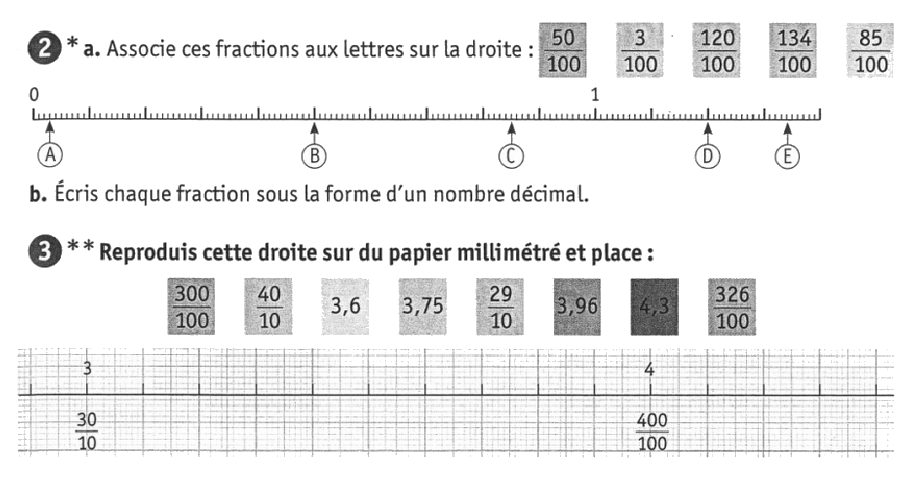
\includegraphics[width=12cm]{Nombres_et_calculs_did/Images/Num4_analyse_droite_sujet}
\end{center}
\vspace*{-8mm}
\begin{enumerate}
   \item Un élève a bien réussi la question \ding{203} mais a fait des erreurs à la question \ding{204}. En comparant la présentation et les tâches demandées dans ces deux questions, donner trois raisons pouvant expliquer cette différence de réussite. 
   \item Quelle définition d'un nombre décimal peut-on proposer à l'école élémentaire ?
\end{enumerate}
{\bf SITUATION 2 : Extrait du manuel \og Tribu des maths \fg{} CM2 Magnard (édition 2010)}
\begin{center}
   \fbox{
   \begin{minipage}{12cm}
   Fatou dit qu'elle a réussi à tracer un segment dont la mesure en décimètres est comprise entre $2+\dfrac{5}{10}+\dfrac{2}{100}$ et $2+\dfrac{6}{10}+\dfrac{1}{100}$. \\
   \medskip
   Max lui dit que ce n'est pas possible, car $\dfrac{1}{100}$ est plus petit que $\dfrac{2}{100}$. \\
   \medskip
   Qui a tort ? Expliquez pourquoi.
   \end{minipage}}
\end{center}
Trois copies d'élèves sont proposées : 
\begin{center}
   \fbox{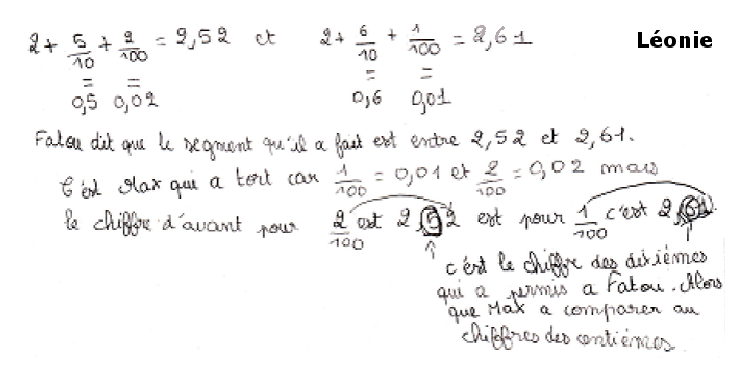
\includegraphics[width=11cm]{Nombres_et_calculs_did/Images/Num4_analyse_droite_Leonie}} \\
   \hspace*{-0.5cm}
   \fbox{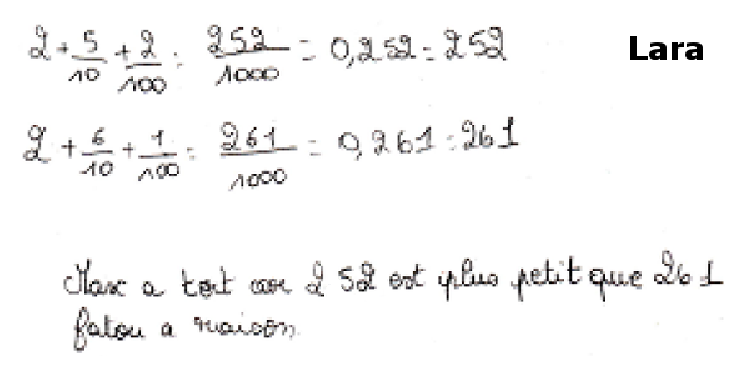
\includegraphics[width=7cm]{Nombres_et_calculs_did/Images/Num4_analyse_droite_Lara}}
   \fbox{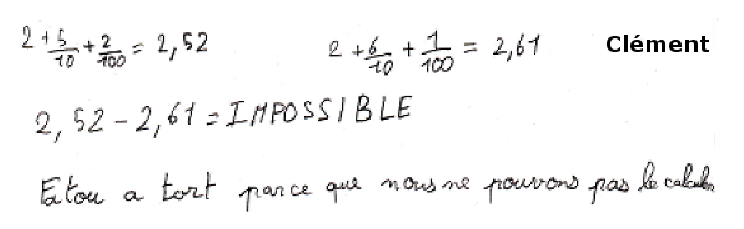
\includegraphics[width=10cm]{Nombres_et_calculs_did/Images/Num4_analyse_droite_Clement}}\hspace*{-0.5cm}
\end{center}
\begin{enumerate}
   \item Quelles sont les erreurs faites par Lara ? Indiquer pour chacune une origine possible.
   \item Citer une compétence qui semble acquise dans le domaine de la numération pour Clément.
   \item Léonie s'appuie sur les écritures décimales des nombres $2+\dfrac{5}{10}+\dfrac{2}{100}$ et $2+\dfrac{6}{10}+\dfrac{1}{100}$ pour comparer ces nombres. Énoncer la règle de comparaison qu'elle utilise implicitement.
\end{enumerate}
\end{exercice}

\begin{corrige}
{\bf SITUATION 1 :} \\
\begin{enumerate}
   \item {\it Voir tableau de comparaison page suivante.} \\
   On peut évoquer plusieurs raisons à la non réussite de l'élèves à la question \ding{204} :
   \begin{itemize}
      \item dans la question \ding{203}, les fractions peuvent être classées facilement dans l'ordre croissant puisqu'elles ont le même dénominateur. Il suffit ensuite de les mettre dans le même ordre sur l'axe gradué étant donné qu'il y a autant de fractions que de lettres. Dans la question \ding{204}, la question est beaucoup plus ouverte ;
      \item la reproduction de la droite elle-même sur du papier millimétré dans la question \ding{204} peut poser problème, d'autant plus que l'origine n'est pas représentée. Dans la question \ding{203}, la droite graduée est déjà tracée ;
      \item dans la question \ding{204}, l'élève doit constamment \og jongler \fg{} entre les différentes écritures, alors que la question \ding{203} ne comprend qu'une sorte d'écriture ;
      \item les deux représentations de 3 et 4 dans l'exercice \ding{204} possèdent des dénominateurs différents, ce qui peut perturber l'élève ;
      \item dans l'exercice \ding{204}, les graduations des centièmes ne sont pas clairement marquées, il faut se servir du papier millimétré comportant de multiples graduations alors que dans la question \ding{203}, les graduations sont claires.
   \end{itemize}
   \item Un nombre décimal est un nombre pouvant s'écrire sous la forme d'une fraction décimale, c'est à dire une fraction dont le dénominateur est une puissance de 10 : 1, 10, 100, 1000\dots \\
\end{enumerate} 

\Coupe
   \begin{Ltableau}{1\linewidth}{2}{p{7.65cm}|p{7.65cm}}
      \hline
      Question \ding{203} & Question \ding{204} \\
      \hline
      \multicolumn{2}{|c|}{Comparaison de la présentation} \\
      \hdashline
      Un droite graduée est tracée, les graduations jusqu'au centième bien représentées. \newline
      La droite comporte l'origine et l'unité. \newline
      Des lettres indiquent des fractions à placer, il y a autant de lettres que de fractions. \newline
      Les nombres à placer sont tous écrits sous la forme d'un fraction décimale de dénominateur 100.
      & La droite doit être reproduite sur papier millimétré. \newline
      \newline
      L'origine n'est pas présente, le premier entier visible est 3. \newline
      3 est associé à $\dfrac{30}{10}$ et 4 à $\dfrac{400}{100}$. \newline
      Les nombres à placer sont des nombres décimaux écrits de différentes façons. \\
      \hline
      \multicolumn{2}{|c|}{Comparaison de la tâche demandée} \\
      \hdashline
      Il s'agit d'associer une fraction à une lettre de la droite graduée. L'élève doit ensuite donner l'écriture décimale de chacune des fractions. 
      & Il faut placer des fractions après avoir reproduit la droite. Il n'y a rien à faire après avoir placé les nombres. \\ 
      \hline
   \end{Ltableau}

\bigskip

{\bf SITUATION 2 }: \\
\begin{enumerate}
   \item {\bf Lara} n'obtient pas le bon dénominateur : elle écrit $1\,000$ au lieu de 100. Cela provient peut-être du fait du codage usuel de $a+\dfrac{b}{10}+\dfrac{c}{100} =\overline{a,bc}$ qu'elle a vu en classe, le $1\,000$ provenant de la suite $1 ; 10 ; 100 ; 1\,000$ ou de la multiplication de $10$ par $100$ ? Ensuite elle se trompe en enlevant la virgule. Il s'agit peut-être d'une manière implicite de comparer les parties décimales \og comme si un nombre décimal était composé de deux nombres entiers séparés par une virgule \fg. Sa conclusion ne justifie pas pourquoi Max à tort.
   \item {\bf Clément} semble avoir acquis la compétence \og passer du développement en factions décimales d'un nombre à son écriture décimale \fg.
   \item Elle utilise la règle suivante : pour comparer deux nombres décimaux, on compare tout d'abord les parties entières. Si l'une est plus grande que l'autre, il en est de même pour le nombre décimal. Si les parties entières sont égales, on compare le chiffre des dixièmes : le nombre le plus grand est celui qui a le plus grand chiffre des dixièmes. On continue ainsi de suite pour chacun des rangs successifs.
\end{enumerate}
\end{corrige}

\bigskip

\begin{exercice}[CRPE 2015 G3]
L'exercice suivant a été donné à des élèves de l'école primaire :
\vspace*{-6mm}
\begin{center}
   \fbox{\begin{minipage}{17cm}
      On découpe un ruban mesurant 137,6 cm en 8 morceaux de même longueur. Combien mesure chacun des morceaux ?
   \end{minipage}}
\end{center}
\vspace*{-6mm}
\begin{enumerate}
   \item Quel sens de la division illustre-t-il ?
   \item Proposer une procédure pour résoudre ce problème, permettant de se ramener à une opération sur les nombres entiers.
   \item Proposer une procédure de calcul qui peut être attendue d'un élève de CM2 pour
effectuer la division $137,6\div8$, sans se ramener à une opération sur les entiers.
   \item Le quotient d'un nombre décimal par 8 est-il toujours un nombre décimal ? justifier.
\end{enumerate}
\end{exercice}

\begin{corrige}
\ \\ [-5mm]
\begin{enumerate}
   \item Il s'agit d'une situation de partage équitable pour laquelle on recherche \og la valeur de chaque part \fg, il s'agit donc d'une division-partition.
   \item Il faudrait pour cela que le dividende soit un nombre entier. Étant donné qu'il est exprimé en cm, il suffit de l'exprimer en mm. On aurait alors un ruban de 1\,376 mm à partager en 8 morceaux de même longueur, soit $1\,736\div8$, exprimée en mm : $\opdiv{1376}{8}$. \quad Chaque morceau mesure 172 mm, soit 17,2 cm.
   \item Au CM2, la procédure experte de la division d'un nombre décimal par un nombre entier est au programme :
   $\opdiv[shiftdecimalsep=divisor]{137,6}{8}$.
   \item Un nombre décimal (positif) peut s'écrire sous la forme $\dfrac{p}{10^q}$ où $p$ et $q$ sont des nombres entiers positifs. \\
   Or, $\dfrac{p}{10^q}\div8 =\dfrac{p}{10^q\times2^3} =\dfrac{p\times5^3}{10^{q}\times10^3} =\dfrac{125p}{10^{q+3}}$ qui est un nombre décimal. \\ [1mm]
   Le quotient d'un décimal par 8 est donc toujours un décimal.
\end{enumerate}
\end{corrige}

\bigskip


\begin{exercice}[CRPE 2017 G2]
Les problèmes suivants, issus du manuel EuroMaths CM2 (éditions Hatier, 2009), ont été donnés en fin d’année à des élèves d’une classe de CM2. La calculatrice n’était pas autorisée.
\begin{center}
\fbox{
   \begin{minipage}{14cm}
   \begin{enumerate}
      \item Un croissant coûte 1,25 \euro. Quel est le prix de 10 croissants ?
      \item Pour 10 baguettes, Pierre paie 8,50 \euro. Quel est le prix d’une baguette ?
      \item Un paquet de 100 enveloppes illustrées coûte 13 \euro. Quel est le prix d’une enveloppe ?
      \item Éric fait la collection de fourmis en plastique. Il en a plus de 100. Chacune de ses fourmis mesure 0,7 cm. Quelle est la mesure de la ligne formée par 100 fourmis à la queue leu leu ? 
   \end{enumerate}
\end{minipage}
}
\end{center}
\vspace*{-2mm}
\begin{enumerate}
   \item Citer deux compétences travaillées dans ces exercices.
   \item Voici les productions de deux élèves en réponse au problème 4.
   \begin{center}
      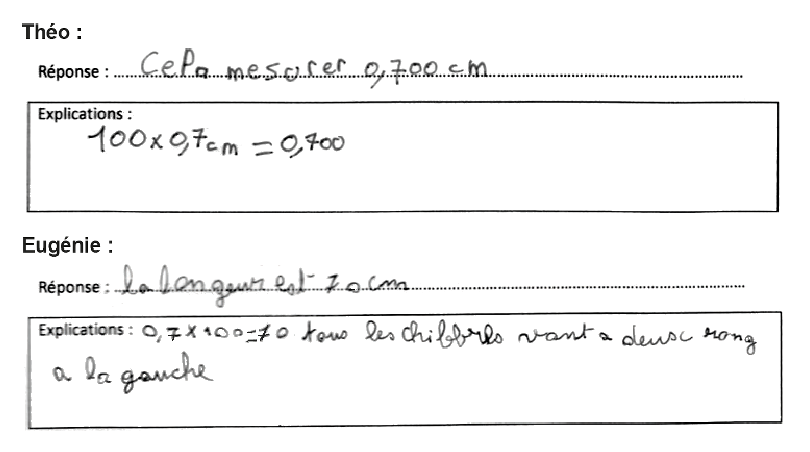
\includegraphics[width=11cm]{{Nombres_et_calculs_did/Images/Num4_analyse_Theo_Eugenie}}
   \end{center}
   \vspace*{-5mm}
   \begin{enumerate}
      \item Analyser l’erreur de Théo en émettant une hypothèse sur son origine.
      \item Formuler précisément la procédure utilisée par Eugénie et en donner une justification mathématique.
   \end{enumerate}
\end{enumerate}
\end{exercice}

\begin{corrige}
\ \\ [-5mm]
\begin{enumerate}
   \item La compétence générale est \og Résoudre un problème de proportionnalité dans le champ multiplicatif \fg{}, à partir à chaque fois d'une valeur unitaire. \\
   Une compétence mathématiques est la maitrise des nombres décimaux et en particulier savoir diviser et multiplier un nombre par 10 et par 100.
   \item
   \begin{enumerate}
      \item {\bf Théo} utilise une règle valable avec les nombres entiers : \og pour multiplier un nombre par 100, on ajoute deux zéros à la fin du nombre \fg{}. \\
      Cependant, cette règle ne s'applique pas aux nombres décimaux, puisqu'ajouter des \og zéros \fg{} à la partie décimale ne change rien à la valeur du nombre.
      \item {\bf Eugénie} a compris que multiplier par 100 revenait à multiplier chaque rang du nombre par 100, c'est-à-dire décaler chaque chiffre de deux rangs vers la gauche dans le tableau de numération. \\
      Cette procédure est meilleure mathématiquement et didactiquement beaucoup plus pertinente que la précédente !
   \end{enumerate}
\end{enumerate}
\end{corrige}

\bigskip


\begin{exercice}[CRPE 2018 G1]
Des élèves d’une classe de cycle 3 doivent calculer $3,12+5,7$ et expliquer comment ils procèdent. \\
Voici des exemples de productions d’élèves :
\begin{center}
   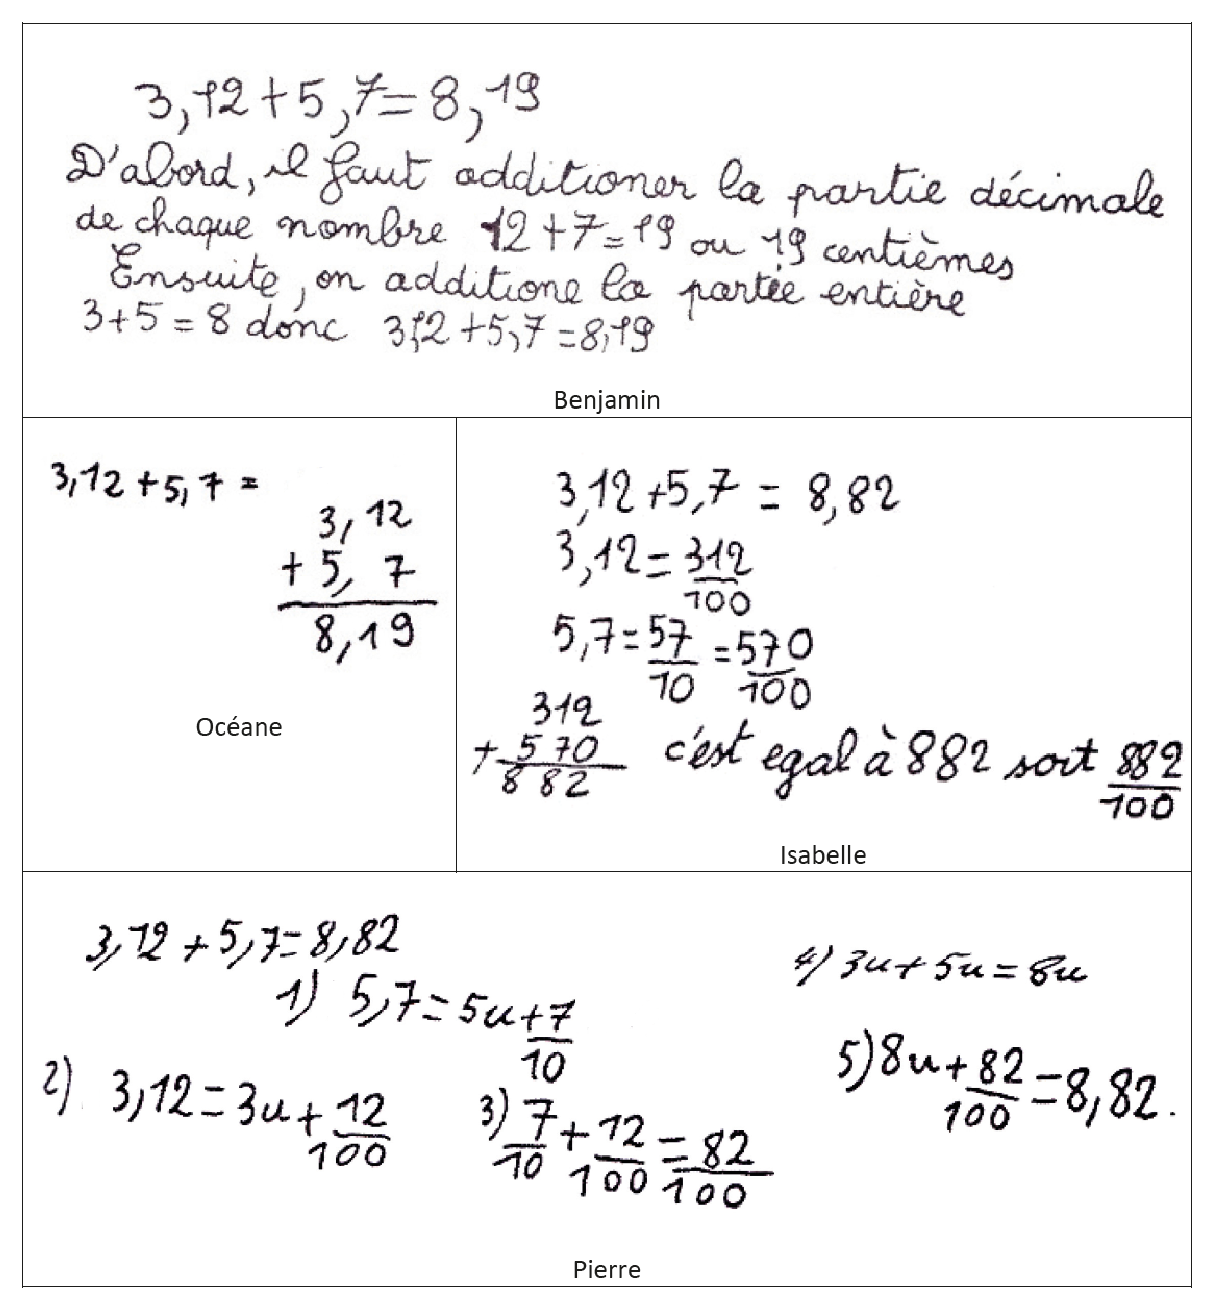
\includegraphics[width=10cm]{{Nombres_et_calculs_did/Images/Num4_analyse_312_57}}
\end{center}
\begin{enumerate}
   \item À partir de l’analyse des différentes productions, expliquer quelles sont les différentes démarches proposées.
   \item Quelle représentation erronée des nombres décimaux pourrait être à l’origine des erreurs des élèves ?
   \item Proposer trois tâches ou activités que pourrait mettre en place l’enseignant pour remédier à ce type d’erreurs ?
\end{enumerate}
\end{exercice}

\begin{corrige}
\ \\ [-5mm]
\begin{enumerate}
   \item Il y a trois démarches principales :
   \begin{itemize}
      \item celle de Benjamin et d'Océane qui calculent séparément la partie entière et la partie décimale soit par des calculs en ligne pour Benjamin, soit par un calcul posé en colonnes pour Océane. Ensuite, ils associent leurs résultats en plaçant une virgule entre les deux.
      \item celle d'Isabelle qui passe par les fractions décimales : elle transforme ses nombres décimaux en fractions décimales de dénominateur 100 afin d'harmoniser les écritures pour pouvoir ensuite en faire une somme unique.
      \item celle de Pierre, une solution hybride qui consiste à décoder ses nombres décimaux en une somme d'un entier (unité) et d'une fraction décimale, puis il effectue des calculs séparés sur les fractions, puis sur les entiers, et enfin il ajoute ses résultats pour pouvoir obtenir un nombre en écriture décimale.
   \end{itemize}
   \item Pour Benjamin et Olivier, ils pensent les nombres entiers décimaux comme deux nombres séparés par une virgule, sans lien entre les deux.
   \item On peut utiliser un instrument de calcul comme des abaques (bouliers ou abaques à jetons) afin d'avoir une représentation plus visuelle du nombre, ce qui a également l'avantage de travailler sur la manipulation et sur l'aspect historique du calcul posé ; on peut également utiliser un tableau de numération et placer les nombres dans le tableau ; enfin, l'enseignant peur revenir à la manière dont ont été introduits les nombres décimaux par les fractions décimales et oraliser les nombres du type \og 3 et 12 centièmes \fg{} au lieu de \og 3 virgule 12 \fg{}.
\end{enumerate}
\end{corrige}


%%%%%%%%%%%%%%%%%%%%%%%%%%
%%%%%%%%%%%%%%%%%%%%%%%%%%
\Recreation

\setcounter{exercice}{0}

{\it Ces exemples d'activités sont inspirées des documents d'accompagnement \og Fractions et décimaux au cycle 3 \fg{} proposés sur le site édu{\bf scol}} [edu3]. \\

\begin{exercice*}[\fbox{C3} - Découverte des fractions simples avec des réglettes Cuisenaire]
   \begin{minipage}{8cm}
      On utilise ici des réglettes Cuisenaire, ou des bandes de papier plastifiées. \\
      Ce matériel a été inventé par un pédagogue belge {\it Georges Cuisenaire} en 1945 sous la forme de réglettes en bois. Il permet, en définissant une unité parmi les réglettes, de travailler et d’entretenir la notion de fraction simple (entre autre). \\
      Différentes activités peuvent être menées avec les élèves. Site Internet (avec vidéos et tutoriels) : \\
      \href{http://www.cuisenaire.eu}{http://www.cuisenaire.eu}
   \end{minipage}
   \qquad
   \begin{minipage}{7cm}
      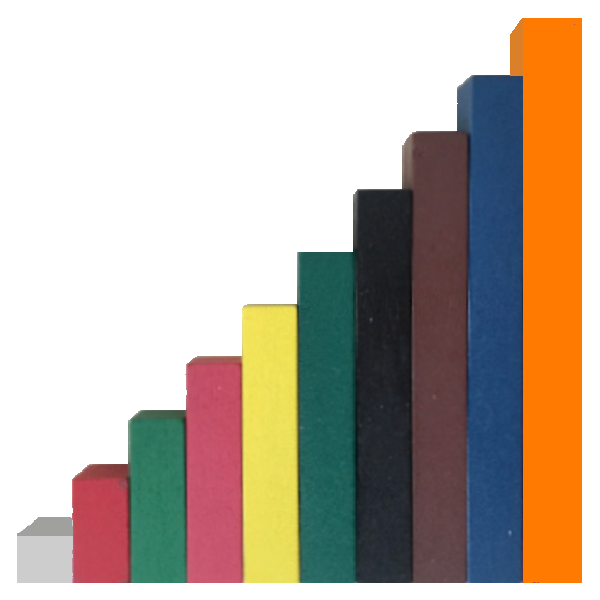
\includegraphics[width=7cm]{Nombres_et_calculs_did/Images/Num4_activites_Cuisenaire}
   \end{minipage} \\ [2mm]
   
   \bigskip
   
{\bf Activité 1 : l'unité est la plus grande des réglettes.} \\
   L'unité est définie comme étant la longueur de la réglette orange. On demande aux élèves de trouver la longueur des réglettes jaunes, rouges et blanches en fonction de cette unité. \\
Par exemple, pour trouver la longueur de la réglette rouge, l’élève regarde combien de ces réglettes sont nécessaires pour reconstituer l’unité : il faut 5 réglettes rouges pour obtenir une unité ; l’unité est donc partagée en cinq parts égales, et une réglette rouge représente une de ces parts. Chaque réglette rouge vaut donc un cinquième de l'unité. \\ [2mm]
   \begin{minipage}{10cm}
            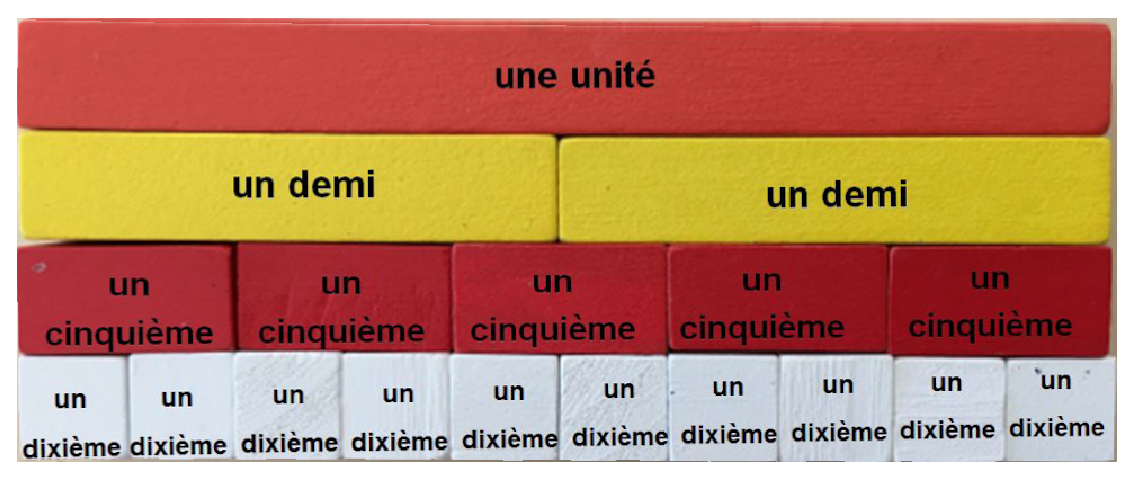
\includegraphics[width=10cm]{Nombres_et_calculs_did/Images/Num4_activites_Cuisenaire_A1}
   \end{minipage}
   \quad
   \begin{minipage}{6cm}
      \begin{itemize}
         \item Jaune : $\frac12+\frac12 =1$ ou $2\times\frac12 =1$ \medskip
         \item Rouge : $\frac15+\frac15+\frac15+\frac15+\frac15 =1$ \\ [1mm] ou  $5\times\frac15 =1$ \medskip
         \item Blanche : $\frac1{10}+\frac1{10}+\frac1{10}+\frac1{10}+\frac1{10}+\frac1{10}+\frac1{10}+\frac1{10}+\frac1{10}+\frac1{10} =1$  \\ [1mm] ou $10\times\frac1{10} =1$
      \end{itemize}
   \end{minipage}
   
   \bigskip
   
{\bf Activité 2 : utilisation d'une unité différente.} \\
   Faire varier l’unité de référence permet de montrer que l’unité n’est pas attachée à un objet singulier. \\
   L’unité est définie maintenant comme étant la longueur de la réglette bleue, il s’agit de trouver la longueur des réglettes vertes et blanche. \\ [2mm]
   \begin{minipage}{9cm}
            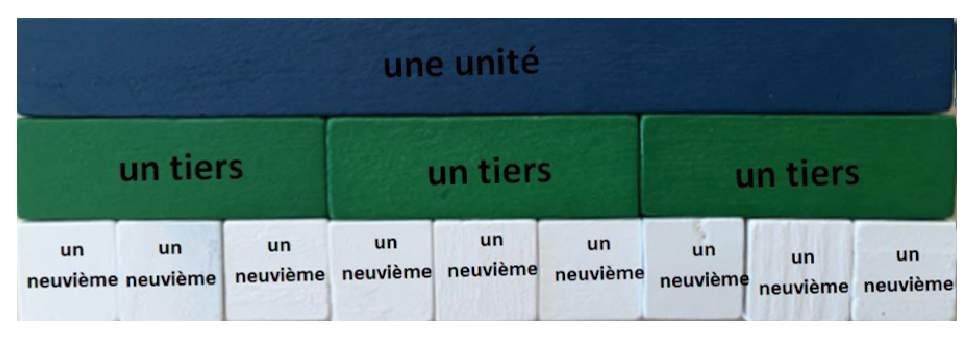
\includegraphics[width=9cm]{Nombres_et_calculs_did/Images/Num4_activites_Cuisenaire_A2}
   \end{minipage}
   \quad
   \begin{minipage}{8cm}
      \begin{itemize}
         \item Verte : $\frac13+\frac13+\dfrac13 =1$ ou $3\times\frac13 =1$ \medskip
         \item Blanche : $\frac1{9}+\frac1{9}+\frac1{9}+\frac1{9}+\frac1{9}+\frac1{9}+\frac1{9}+\frac1{9}+\frac1{9}+\frac1{9} =1$  \\ [1mm] ou $9\times\frac1{9} =1$
      \end{itemize}
   \end{minipage}
   
   \pagebreak
   
{\bf Activité 3 : fractions supérieures à 1.} \\
   La réglette orange vaut maintenant deux unités, il s'agit de trouver la longueur des réglettes jaunes, blanches, marron et roses.
   \begin{center}
         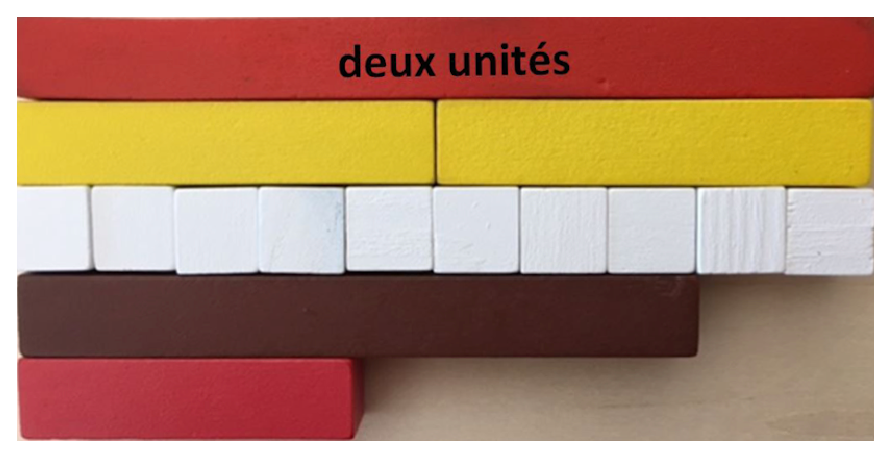
\includegraphics[width=10cm]{Nombres_et_calculs_did/Images/Num4_activites_Cuisenaire_A3}
   \end{center}
   Laisser les élèves produire des phrases et écritures différentes en leur imposant de se rapporter à l'unité. Par exemple :
   \begin{itemize}
      \item La réglette jaune vaut une unité.
      \item Chaque réglette blanche correspond au cinquième de l’unité.
      \item La réglette marron vaut une unité plus trois cinquièmes de l’unité, ou encore huit cinquièmes de l’unité ou deux unités moins deux cinquièmes de l’unité.
      \item La réglette rose vaut quatre cinquièmes ou la moitié de huit cinquièmes ou une unité moins un cinquième.
   \end{itemize}
La compétence \og représenter \fg{} est développée ici au travers de la production de diverses écritures de fractions simples. \\

{\bf Activité 4 : travail inverse.} \\
   On travail la compétence inverse : à partir de la fraction, il s'agit de retrouver l'unité. \\ [2mm] 
   La réglette blanche vaut un septième de l’unité, quelle est l’unité ? \\ [2mm]
   \begin{minipage}{7cm}
      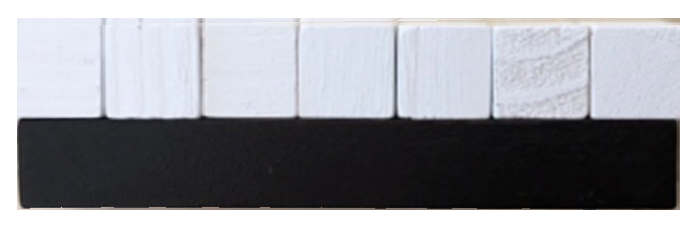
\includegraphics[width=7cm]{Nombres_et_calculs_did/Images/Num4_activites_Cuisenaire_A4}
   \end{minipage}
   \qquad
   \begin{minipage}{9cm}
      Pour obtenir un septième, on a dû partager l’unité en sept parts égales. Pour retrouver l’unité, il faut donc prendre 7 fois un septième. \\ [1mm]
      $\frac17+\frac17+\frac17+\frac17+\frac17+\frac17+\frac17 =1$ 
   \end{minipage}
   
   \medskip
   
   La réglette verte vaut $\dfrac34$  de l’unité, quelle est l’unité ? \\ [2mm]
   \begin{minipage}{8cm}
      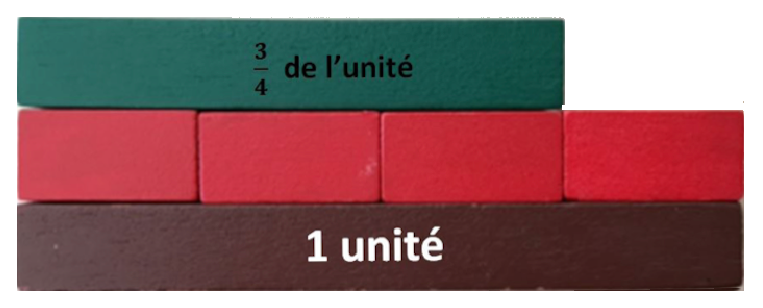
\includegraphics[width=8cm]{Nombres_et_calculs_did/Images/Num4_activites_Cuisenaire_A5}
   \end{minipage}
   \qquad
   \begin{minipage}{8cm}
      Pour obtenir $\frac34$ de l’unité, on a partagé l’unité en 4 parts égales et on a pris 3 de ces parts. La réglette verte représente ces 3 parts. Je cherche la réglette qui peut représenter l’une de ces 3 parts : il s’agit de la réglette rouge (car trois réglettes rouges valent une réglette verte). La réglette unité est donc la réglette marron.
   \end{minipage}
\end{exercice*}


\pagebreak

\begin{exercice*}[\fbox{C3} - De la fraction simple à la fraction décimale]
   \bigskip
   {\bf Activité 1 : la bande graduée.} \\
   Les élèves disposent de baguettes de bois identiques partagées en 10 parts égales, de bandes de papier de différentes longueurs, ainsi que d’une affiche pour y inscrire le résultat de leur recherche. \\
La règle graduée n’est pas autorisée. Les élèves travaillent par groupe. Une baguette et une bande sont distribuées à chaque groupe et la consigne est la suivante :
\begin{center}
   \fbox{\parbox{12cm}{L’unité choisie est la longueur de la règle en bois. Vous devez mesurer la longueur de la bande de papier à l’aide cette unité. Vous pouvez donner plusieurs réponses. Lorsque vous vous êtes mis d’accord, écrivez vos réponses sur l’affiche.}}
\end{center}
Après un temps de recherche suffisant pour que chaque groupe parvienne à donner au moins une réponse, une première mise en commun est menée avec la classe. Chaque groupe vient commenter au tableau son affiche et expliquer sa façon de procéder. \\
Ce peut être le moment pour la classe de se mettre d’accord sur la réponse attendue : par exemple, si groupe a répondu \og la baguette mesure 13 graduations \fg, on peut revenir avec la classe sur la consigne, repréciser l’unité avec laquelle on mesure, et chercher la valeur de l’une des \og graduations \fg.
Une fois cette synthèse intermédiaire menée, chaque groupe termine le travail. Une nouvelle synthèse collective est conduite afin de faire expliciter les procédures et les différentes écritures. Cette activité peut être reprise ultérieurement en donnant des baguettes de longueurs différentes dans chacun des groupes, cela permet de travailler la notion d’unité pour introduire plus tard l’écriture à virgule.
  \begin{center}
      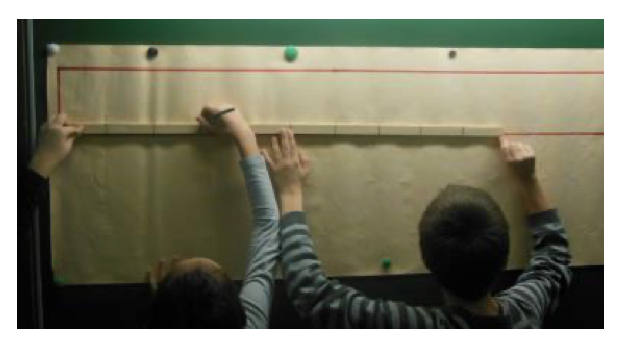
\includegraphics[height=3cm]{Nombres_et_calculs_did/Images/Num4_analyse_bandes_A0}\;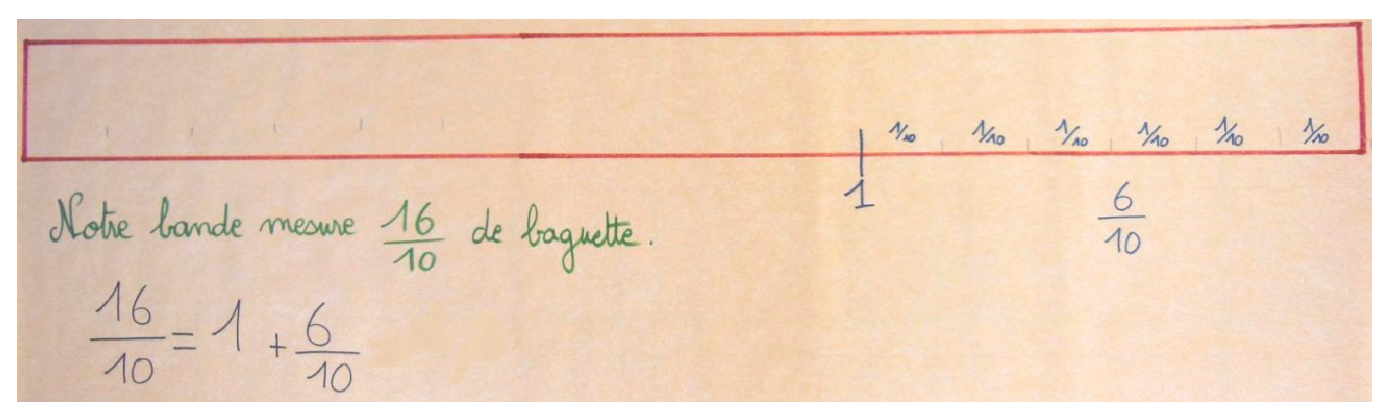
\includegraphics[height=3cm]{Nombres_et_calculs_did/Images/Num4_activites_bandes_A1}
   \end{center}
   
   \bigskip
   
   {\bf Situation 2 : construction de nombres.} \\
Les élèves disposent en plusieurs exemplaires de cartes :
\begin{itemize}
   \item d’unités ;
   \item d’unités partagées en 10 parts égales ;
   \item d’unités partagées en 100 parts égales.
\end{itemize}
\begin{pspicture}(0,0)(5,2.8)
   \psframe[fillstyle=solid,fillcolor=yellow](0,0)(5,2)
   \rput(2.5,1){\Huge\darkgray unité}
   \rput(2.5,2.3){\small\it unité}
\end{pspicture}
\qquad
\begin{pspicture}(0,0)(5,2.8)
   \psframe[fillstyle=solid,fillcolor=green](0,0)(5,2)
   \psgrid[gridlabels=0,subgriddiv=1](0,0)(5,2)
   \rput(2.5,1){\Huge\darkgray unité}
   \rput(2.5,2.3){\small\it unité partagée en 10 parts égales}
\end{pspicture}
\qquad
\begin{pspicture}(0,0)(5,2.8)
   \psframe[fillstyle=solid,fillcolor=cyan](0,0)(5,2)
   \multido{\n=0.25+0.25}{19}{\psline(\n,0)(\n,2)}
   \multido{\n=0.4+0.4}{4}{\psline(0,\n)(5,\n)}
   \rput(2.5,1){\Huge\darkgray unité}
   \rput(2.5,2.3){\small\it unité partagée en 100 parts égales}
\end{pspicture}

Ainsi que de cartes sur lesquelles figurent différents nombres écrits de différentes manières.
\begin{center}
   \fbox{206 centièmes} \qquad \fbox{2 unités et 6 centièmes} \qquad \fbox{$2+\dfrac{6}{100}$} \qquad \fbox{$\dfrac{20}{10}+\dfrac{6}{100}$}\qquad \fbox{$\dfrac{26}{100}$} \qquad \fbox{26 dixièmes}
\end{center}

Les élèves travaillent en groupe. Une seule carte-nombre est distribuée à chaque groupe au début. La tâche consiste en premier lieu à construire le nombre figurant sur la carte à l’aide des unités. \\
Lorsqu’un groupe a terminé, l’enseignant distribue une autre carte. Ce scénario permet une différenciation naturelle : l’objectif est le même pour toute la classe, mais certains groupes pourront construire plus de nombres que d’autres, chacun ayant le temps d’avancer à son rythme. \\
Les élèves collent le nombre construit et la carte-nombre sur une affiche tout en échangeant et en confrontant leurs idées. À l’issue de la recherche, les travaux sont mutualisés et commentés avec la classe et les différentes écritures d’un même nombre sont regroupées ensemble.
\begin{center}
   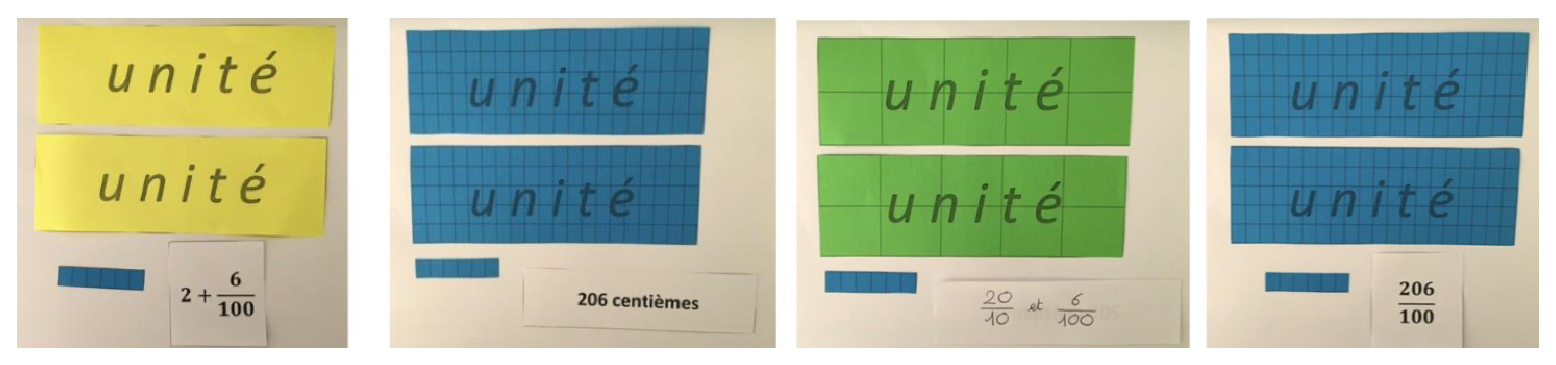
\includegraphics[width=17cm]{Nombres_et_calculs_did/Images/Num4_activites_bandes_A2}
\end{center}
On pourra également afficher des nombres différents mais dont l'écriture est proche ($\dfrac{26}{100}$ et 26 dixièmes par exemple). \\
Une trace écrite est conservée sous la forme d’un affichage dans la classe et dans le cahier des élèves. Dans les cahiers, les élèves notent le par exemple le plus grand nombre d’écritures possibles de 2 unités et 6 centièmes
\begin{center}
   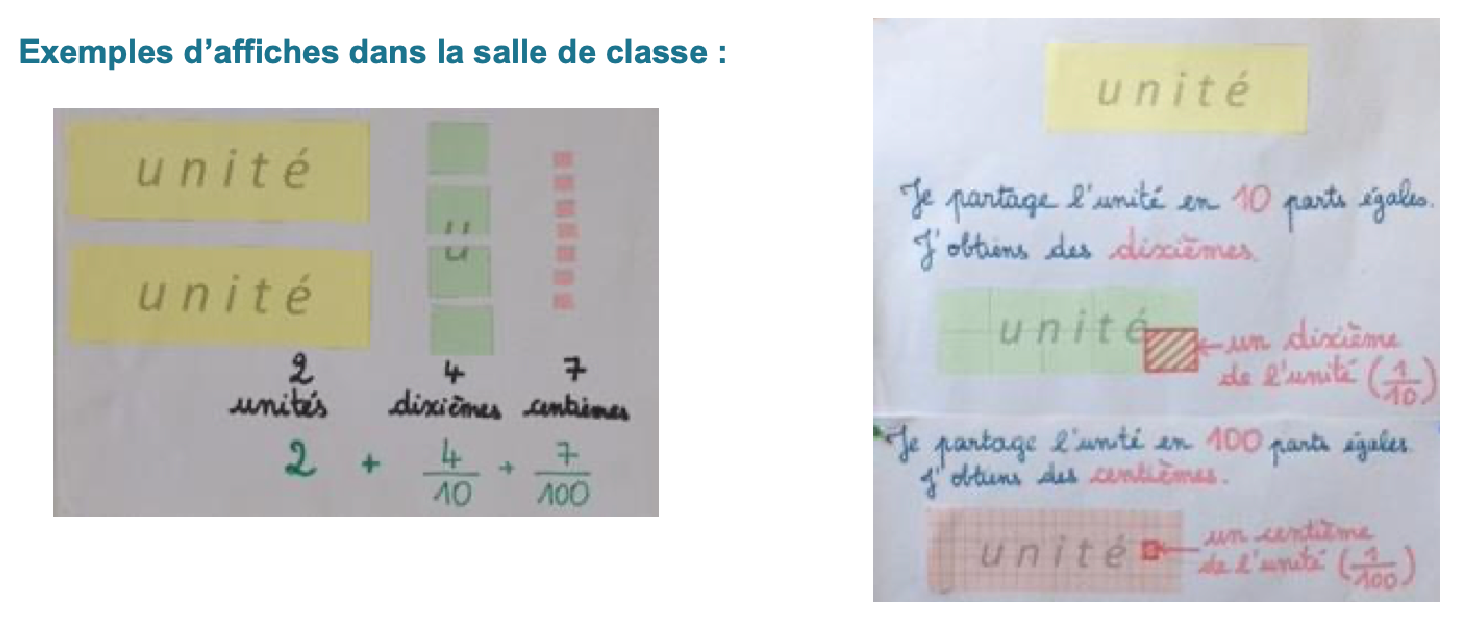
\includegraphics[width=17cm]{Nombres_et_calculs_did/Images/Num4_activites_bandes_A3}
\end{center}
Cette activité permet :
\begin{itemize}
   \item de travailler les équivalences d'écritures ;
   \item elle donne du sens à des écritures différentes ;
   \item elle crée une image mentale des nombres et du rapport 10 entre les différentes unités ;
   \item elle facilite les comparaisons ;
   \item elle peut être complexifiée en ajoutant une unité partagées en millièmes en CM2.
\end{itemize}
\end{exercice*}

\pagebreak

\begin{exercice*}[\fbox{C3} - De l'écriture fractionnaire à l'écriture décimale]
   \bigskip
   On peut reprendre à cette étape les affichages des activités précédentes et y ajouter l'écriture décimale, comme codage de l'écriture sous forme de fractions décimales.\\

   On peut ensuite constituer des \og fleurs des nombres \fg : l’enseignant.e choisit un nombre qui est écrit au centre de la fleur.
Les élèves cherchent individuellement le plus de représentations possibles de ce nombre et une synthèse collective est ensuite effectuée.
\begin{center}
    \includegraphics[width=10cm]{Nombres_et_calculs_did/Images/Num4_analyse_virgule_V2}
\end{center}
Cette situation peut être proposée en fin de séquence, pour permettre des réinvestissements et pour développer des automatismes. Elle peut également être utilisée plus tôt lors des premiers travaux sur les différentes décompositions en sommes de fractions décimales.
En guise de trace écrite, l’élève pourra compléter sa production personnelle avec d’autres écritures proposées par ses camarades.

\begin{center}
   {\psset{unit=1.2}
      \begin{pspicture}(-4,-4)(4,4)  
         \multido{\n=0+60}{6}{\psline(0,0)(3;\n)}
         \multido{\n=30+60,\i=-60+60,\r=120+60}{6}{\psarc(2.6;\n){1.5}{\i}{\r}}
         \pscircle[fillstyle=solid,fillcolor=yellow](0,0){1.3}
         \rput(0,0){\Large\bf 7,92}
         \rput(2.6;30){$7+\dfrac{92}{100}$}
         \rput(2.6;-30){$7+\dfrac{9}{10}+\dfrac{2}{100}$}
         \rput(2.6;-90){$\dfrac{79}{10}+\dfrac{2}{100}$}
         \rput(2.6;-150){\parbox{2cm}{$1\times7+9\times\dfrac{7}{10}+2\times\dfrac{2}{100}$}}
         \rput(2.6;150){\parbox{2cm}{$7\times1+0,1\times9+0,01\times2$}}
         \rput(2.6;90){$\dfrac{7920}{1000}$}
      \end{pspicture}
   }
\end{center}  
\end{exercice*}     

